
\chapter{绪论}
\section{课题的研究背景及意义}

人脑,人体内最复杂且精妙的器官,作为中枢神经系统的最高级组成部分,被视为人类意识的物质载体。它直接主导了人的思想、记忆、情绪、触觉以及运动能力,调节着人体与外界的交互行为\cite{1-1}。人脑主要由神经元和神经胶质细胞组成,这些数量庞大的神经细胞通过向外发送化学与电信号精准的控制着全身的每一个进程,并为接收到的信号给出具体解释——感到喜悦、疲劳或者疼痛等等\cite{1-2}。人脑之所以能够实现对于身体的精准控制,离不开其内部各部分间的分工协同。从广义角度看,人脑分为大脑,脑干以及小脑三部分。而具体来说,这三部分又可以细分为负责运动协调功能的中脑;控制咀嚼,眨眼和面部表情的脑桥;调节心率、呼吸,血流量以及血氧平衡的延髓等不同结构。这些复杂的功能结构以及它们之间的协调联动使得对于人脑的研究成为了自然科学中最具挑战性,同时也是最具魅力的学科之一,吸引了众多科学研究人员。随着对脑科学的探索不断促进着计算机科学、神经影像学、认知心理学以及微观生物学等众多领域的变革与发展,对于人脑的研究已经得到了国家层面的关注。2013年,美国宣布启动“BRAIN Initiative”大脑研究计划,旨在支持类脑技术的开发应用,研究大脑功能和人体行为的复杂联系,找寻应对脑部疾病的新方法。同年十月,欧盟也启动了“Human Brain Project”研究计划,致力于对人脑的大规模模拟,并推进在神经信息学、神经形态计算、高性能计算以及医学信息学等领域的发展研究。在“一体两翼”方针的基础上,历时六年筹划的“中国脑计划”也已于2021年正式启动,其涉及59个不同研究领域与方向,旨在应对脑疾病诊治、脑认知功能以及脑机智能技术等领域所面临的挑战。众多国家以及相关科研人员的努力,让人脑研究步入了日新月异的快车道。

随着脑科学研究的深入,脑内连接(Brain Connectivity)被认为是揭示大脑不同区域功能并理解它们之间复杂的皮层通讯信息的关键\cite{1-3,1-4,1-5}。近年来,越来越多的脑科学研究人员已经将脑内连接作为探索人脑奥秘的主要手段。脑内连接可以细分为神经解剖学连接、功能性连接以及有效连接。其中神经解剖学连接特指通过微观生物学手段获得的神经元尺度上的神经突触或者神经纤维连接\cite{1-3};功能性连接被定义为在远距离空间上神经生理区域之间的统计依赖性\cite{1-10},其通常基于相关性、相干性和信息论方法来进行分析\cite{1-11,1-12,1-8};有效连接则代表了一个神经区域对其他神经区域影响的因果关系,与只分析统计学联系的功能性连接不同,有效连接倾向于揭示神经区域之间交互的潜在机制\cite{1-14},它是动态的,并且依赖于连接模型的\cite{1-15}。功能性连接以及有效连接可以通过磁共振成像(Magnetic Resonance Imaging,MRI)和扩散张量成像(Diffusion Tensor Imaging,DTI)技术,借助其较高的空间分辨率进行获取\cite{1-6,1-7}。然而,高昂的使用成本和极低的时间分辨率限制了这些方法的应用。

基于这一问题,脑电图(Electroencephalography,EEG)——一种具有较高时间分辨率的低成本脑部电生理监测方法走入研究人员的视野。尽管EEG不能直观地反应脑内神经解剖学连接结构,但是其可以被用来评估功能性连接和有效连接。与MRI相比,EEG具有更高的时间分辨率,因此可以在更短的时间尺度内评估脑内连通性。与此同时,EEG能够在临床症状出现以及MRI可观测的脑结构性变化发生之前,以较低的成本对可能影响大脑网络的生理现象做出预测\cite{1-8,1-9}。

考虑到EEG拥有相较于其他脑内连接观测方法更长的生理预测周期以及更强的泛化性,针对其的采集与分析成为了人脑研究的核心之一。而这一切,离不开脑机接口(Brain Computer Interface, BCI)这一关键性概念。BCI是一种通过在人脑(或脑细胞培养物)与外部设备之间建立通路,实现神经系统与电子设备(如计算机、机器人)之间信息交互以及功能融合的技术\cite{1-104,1-101}。基于EEG的非侵入式BCI系统,融合EEG诱发、采集、处理以及分析为一体,使得基于EEG的脑内连接观测成为可能,逐渐成为生物医学研究中的热门领域。近年来,基于EEG的BCI系统已经在医疗、教育、科研以及军事领域得到了成功应用\cite{1-16,1-17,1-18}。

尽管基于EEG的BCI系统已经在近年来得到了长足发展,但是依然存在着两个方面的问题制约着它的落地与推广。首先是硬件方面:虽然EEG已经具有相较于MRI和DTI更低廉的使用成本,但是当前成熟的EEG采集设备价格仍然十分昂贵,并且它们大多体积庞大,操作复杂,难以适应大多数的实际应用环境。其次,是软件方面:现有的EEG分类辨识算法存在着依赖专家设计、泛化能力不足的问题。由于人脑状态随时间会产生大幅波动,并且EEG采集环境也很难在使用中时刻保持恒定,这些算法往往需要使用者根据数据特点进行自主调整。并且通常情况下,调整后的模型也难以在其他类型EEG数据、其他使用者的同类型数据,甚至是相同使用者不同时段的数据上取得能够接受的辨识性能。毫无疑问,这在另一个方面上制约着BCI系统的实际使用效果。

因此,设计一款功能完善、成本低廉、体型较小并且操作便捷的多通道EEG采集设备,配合能够自主设计模型结构,具备强大泛化能力,能够应对不同使用场景的EEG分类辨识模型,对基于EEG的BCI系统发展与推广具有十分重要的意义。

\section{基于EEG的BCI研究现状}
\subsection{基于EEG的BCI系统概述}
BCI是建立在大脑与计算机或外部设备间不涉及肌肉活动的单/双向通信连接\cite{1-100}。其在设计之初被构想为一种用于增强甚至取代现有的神经康复系统,或者能够帮助使用者通过大脑直接控制辅助设备的潜在技术。1973年,J.J.Vidal设计出了基于EEG的非侵入式BCI系统\cite{1-22},这是BCI技术与EEG的首次结合。近年来,EEG-BCI技术的研究应用发展显著,包括提高人类工作效率的睡意检测系统\cite{1-23,3-18}、反应时间估计\cite{1-24}、虚拟现实控制\cite{1-25}、四旋翼飞行器操纵\cite{1-26}以及类人机器人驾驶\cite{1-27}。BCI系统的使用已经涉及到了人类日常生活的方方面面,一个标准的EEG-BCI系统构成如图\ref{fig1-1}所示:

\begin{figure}[h]
	\centering
	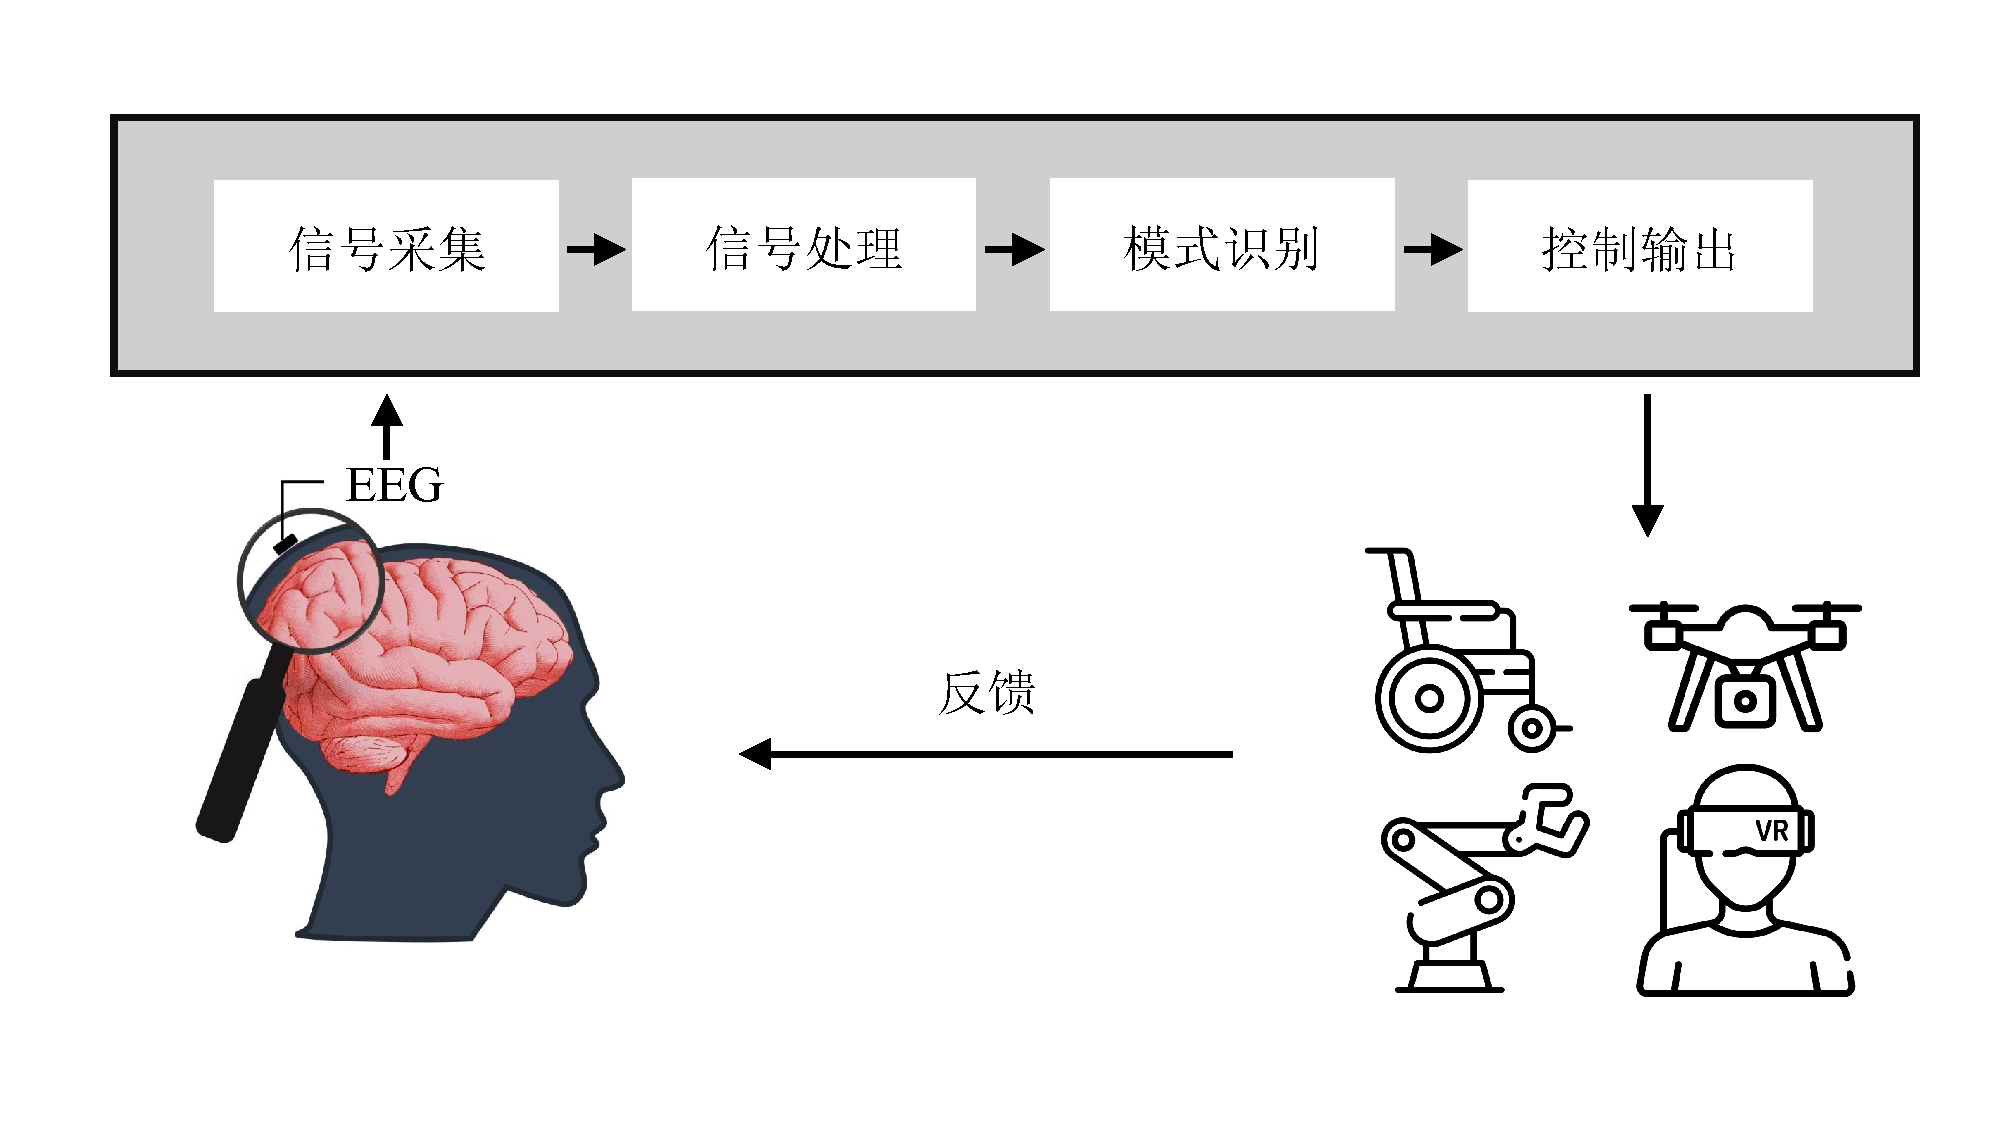
\includegraphics[width=0.5\textheight]{BCI系统构成.pdf}
	\caption{基于EEG的闭环BCI系统\cite{1-28}}
	\label{fig1-1}
\end{figure}

其通常包含四个主要组成部分:信号采集、信号处理、模式识别以及控制输出。当人脑受到特定的外界刺激,或者进行某类具体的思想活动时,其会产生对应类型的EEG信号。这些特定模式的EEG信号会被BCI系统精准获取,在进行适当的滤波降噪以及伪影筛除等预处理步骤后,被送往BCI系统的模式识别模块。模式识别算法通过对预处理后EEG信号进行特征提取,实现对当前人脑状态的预测或者辨识,解码人脑意图,并生成相应的控制指令,进行对外部设备的操控。外部设备的运行结果又会进一步反馈给使用者,从而形成控制闭环。

\subsection{EEG信号基本特征}
EEG作为一种成熟的脑科学研究手段,早在1875年便被英国内科医生Richard Canton首次发现。然而,由于采集设备的限制,直到1924年,
EEG才被德国科学家Hans Berger第一次系统记录下来\cite{1-20}。自此开始,EEG便被用来指代通过电极在人脑头皮表面收集到的生物电信号。这些由电极周围数量庞大的神经元电生理活动所组成的总体反应,包含了庞大的生理信息,是了解脑内连接和辨识大脑状态的有力工具。

由于EEG信号在时域上具有高度的非高斯性、非线性和非平稳性,因此从时域上难以直观地获取有价值的信息\cite{1-21,1-103}。然而,EEG具备十分显著的频域特征,这导致人脑的某些状态往往会与不同的EEG频段直接挂钩。在进行EEG分析时,频域特征是不可或缺的重要信息。一般情况下,人脑EEG信号的频率集中在0.2 Hz至60 Hz之间,并被分为五个主要频段:$\delta$、$\theta$、$\alpha$、$\beta$以及$\gamma$。各频段的常见脑区如图\ref{fig1-2}所示。这五个频段的主要特点如下:

\begin{figure}[!h]
	\centering
	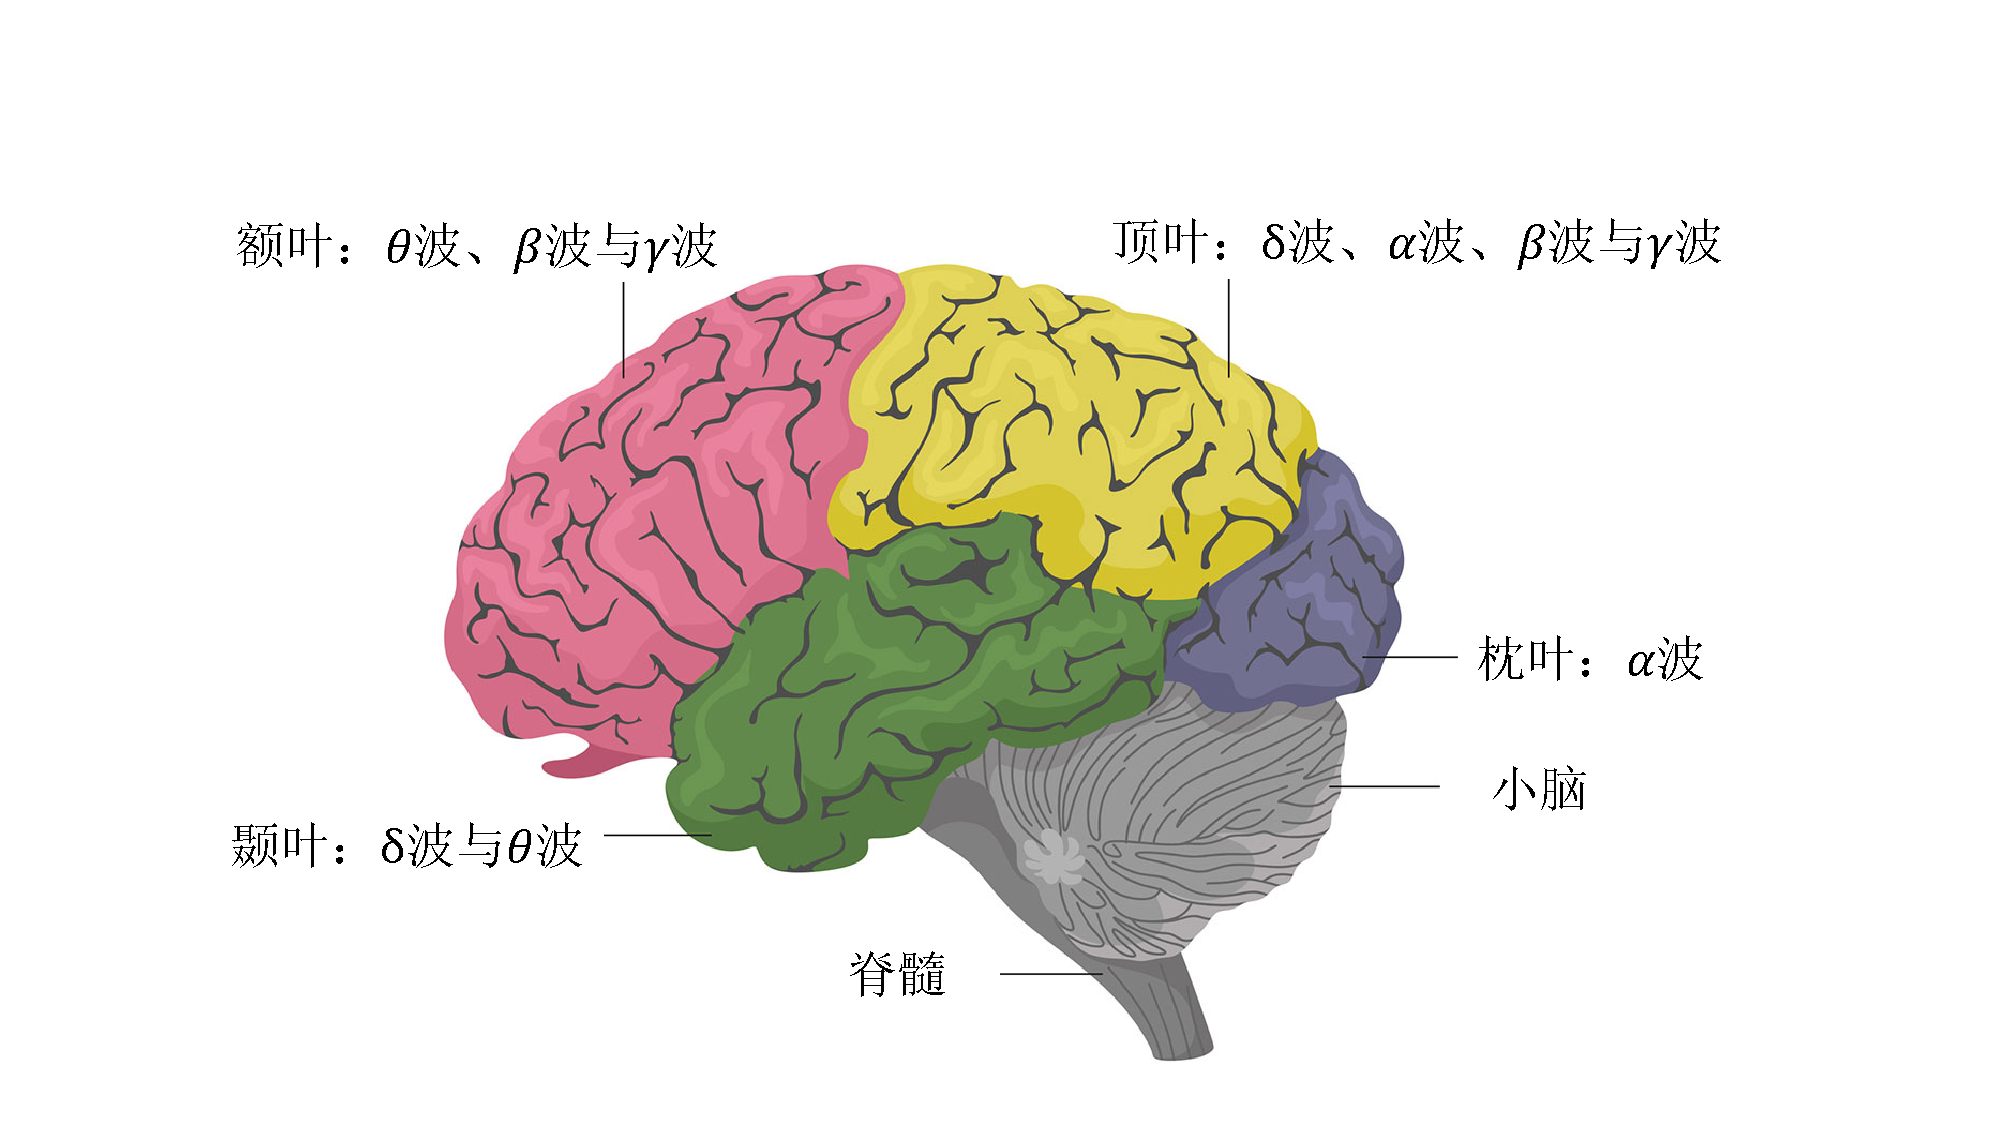
\includegraphics[width=0.45\textheight]{EEG脑区.pdf}
	\caption{不同频段EEG活跃脑区}
	\label{fig1-2}
\end{figure}

$\delta$频段:一般为0.2 Hz-4 Hz,幅值处于20 $\mu $V-150 $\mu $V之间。这一频段的信号通常出现于两类人群:(1) 处于沉睡状态或极度疲劳状态下的成年人颞叶区域,此时幅值相对较低;(2) 大脑尚未发育成熟的婴儿颞叶与部分顶叶区域,此时幅值相对较高。$\delta$频段代表了人体的无意识调节功能,平稳的$\delta$波有助于恢复疲劳,提升机体免疫能力。

$\theta$频段:一般为4 Hz-8 Hz,幅值处于100 $\mu $V-150 $\mu $V之间。$\theta$频段反映了人脑的潜在情绪与体验感受,当人发生情绪波动时会出现在大脑的颞叶和部分额叶区域。$\theta$波也与人脑的精神状态回复具有一定关联性,平稳的$\theta$波有助于提升创造性,放松心态。

$\alpha$频段:一般为8 Hz-13 Hz,幅值处于20 $\mu $V-100 $\mu $V之间。$\alpha$频段为人脑有意识活动与无意识活动的中间地带,是静息态EEG信号的主要成分。在人脑处于理想放松状态时,$\alpha$波将会出现在大脑的顶叶和枕叶区域。

$\beta$频段:一般为13 Hz-30 Hz,幅值处于5 $\mu $V-20 $\mu $V之间。$\beta$频段代表了人脑的有意识活动,在认知、推理、计算、阅读以及理解等任务中扮演着重要角色。$\beta$频段是人脑处于清醒状态下的主要频段,因此当其活动增强时,大脑会自动降低$\alpha$频段活跃程度。$\beta$波常见于大脑的额顶叶区域。

$\gamma$频段:一般为30 Hz-60 Hz,幅值活动范围较大。$\gamma$频段在人脑的学习与记忆环节常常发挥重要作用,高活跃度的$\gamma$波代表了个体具有较强的学习适应能力。当人脑处于记忆、学习以及冥想中时,$\gamma$波通常出现在额叶和额顶叶区域。

深入了解EEG基本特征,有助于BCI系统的合理搭建,并能够帮助BCI系统提升人脑状态辨识与控制意图解码的准确性。


\subsection{基于EEG的BCI系统范式}
为了将基于EEG的BCI系统应用于具体的现实环境,必须为实验的所有阶段选择特定的协议和范式。具体来说,使用者首先需要执行一个特定的任务(比如想象任务或者视觉任务),以学习如何调节他们的大脑活动,此时BCI会记录使用者的EEG信号。这些采集得到的信号将被作为训练数据,以生成该范式的神经解码器(模式识别算法)。之后,当使用者再次执行同类任务时,训练好的神经解码器便能成功进行BCI控制。

常见的EEG-BCI系统范式包括:稳态视觉诱发电位(Steady State Visual Evoked Potential,SSVEP)范式\cite{1-29,1-30}、事件相关电位(Event-Related Potentials,ERP)范式\cite{1-31,1-32}、运动想象(Motor Imagery,MI)范式\cite{1-33,1-34}和被动范式(Passive Paradigm)\cite{1-35}。
 
(1) 基于SSVEP范式的BCI系统

\begin{figure}[!h]
	\centering
	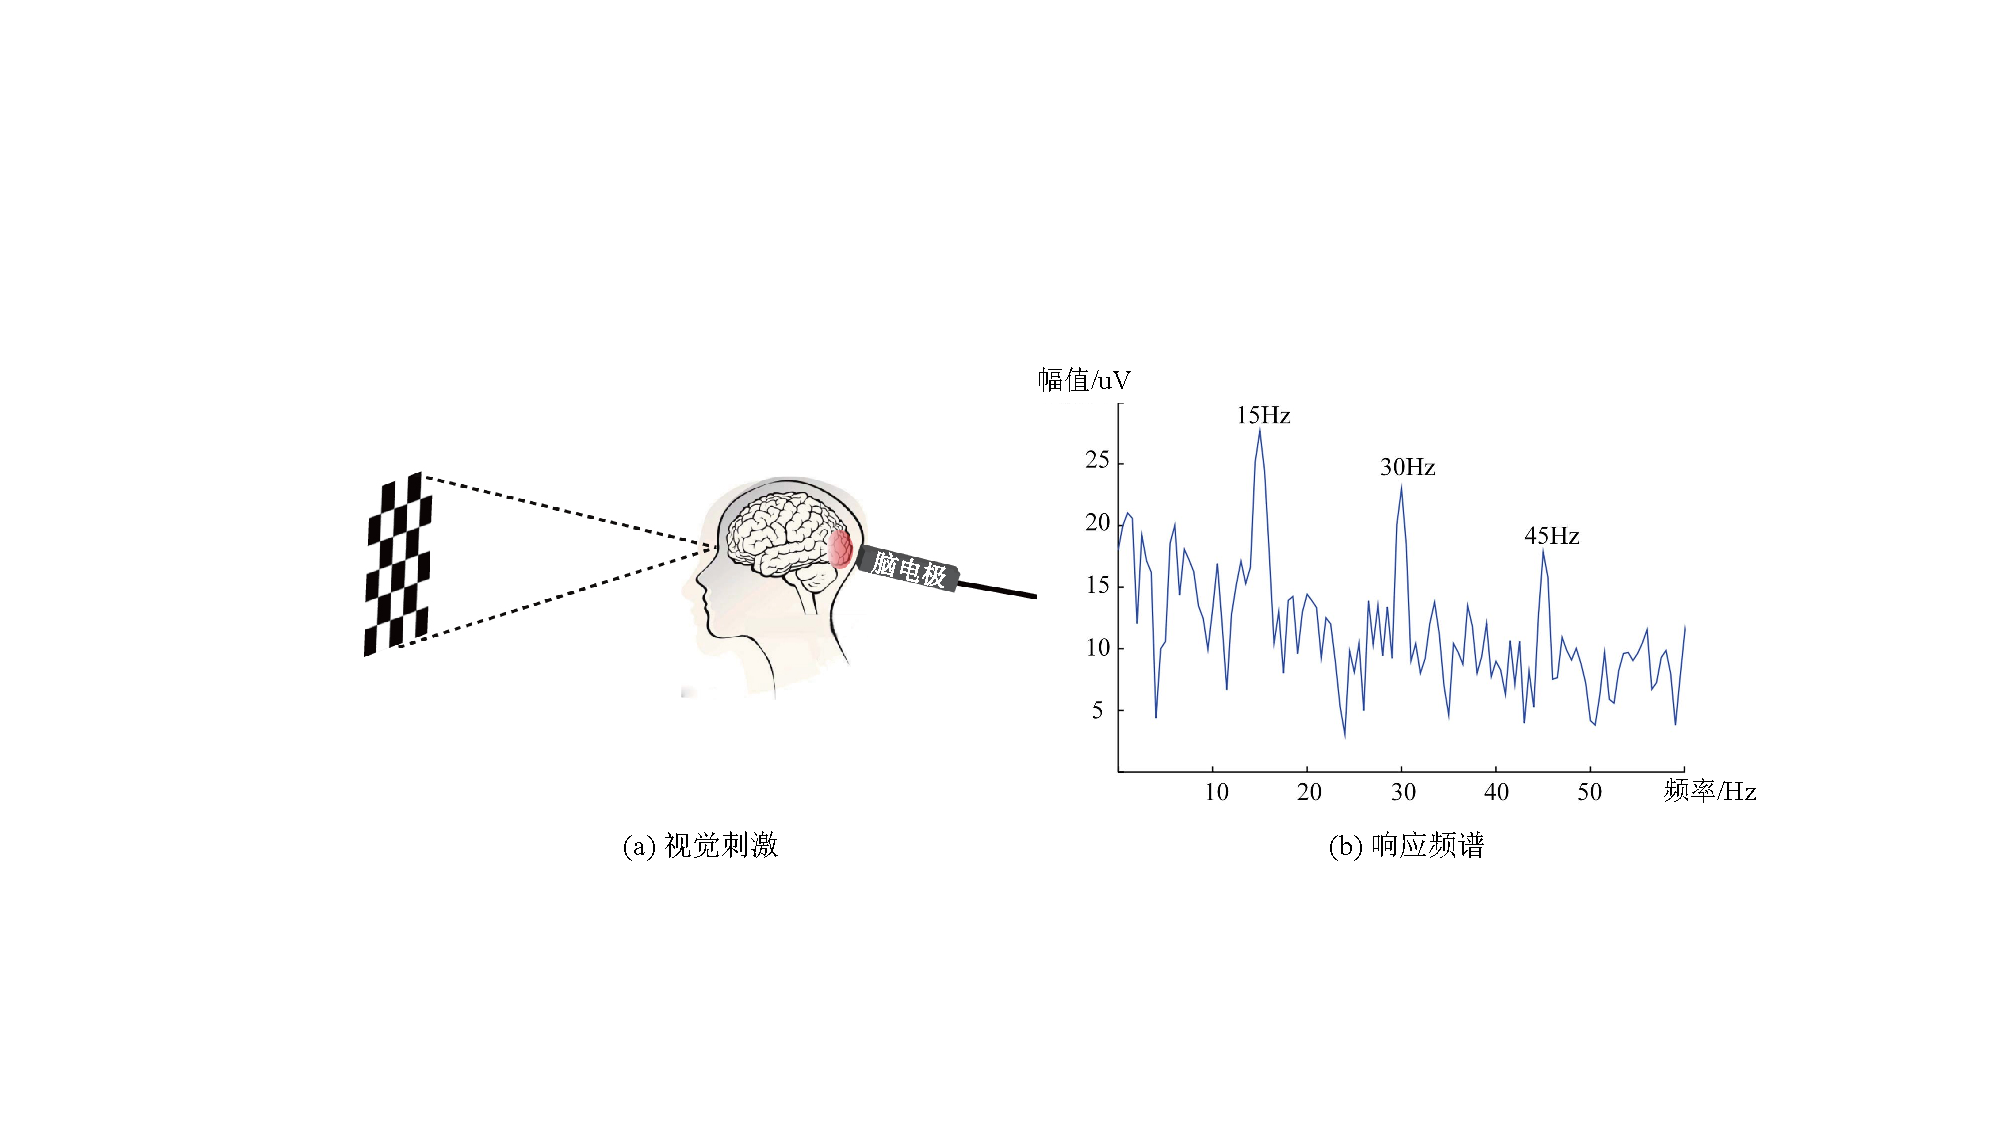
\includegraphics[width=0.61\textheight]{SSVEP.pdf}
	\caption{基于SSVEP范式的BCI系统}
	\label{fig1-3}
\end{figure}

SSVEP在诱发时,需要使用者将目光和注意力转移到闪烁的刺激源上,以唤起视觉皮层的电位响应,因此SSVEP范式又被称作光电驱动EEG(Photic Driving EEG)。在SSVEP范式中,投射到视网膜中央的恒定频率闪烁刺激会在人脑中产生与闪烁源频率相同的EEG信号。闪烁源的刺激频率可以在低频(1 Hz-3.5 Hz)到高频(75 Hz-100 Hz)范围内任意选择\cite{1-37}。闪烁刺激可以通过发光二极管或阴极射线管产生。在使用时,通过向使用者展示具有不同闪烁频率的多个闪烁目标,唤起使用者不同频段的EEG响应,之后通过EEG的频域特征来辨识使用者的观察意图。SSVEP范式的BCI系统实验内容如图\ref{fig1-3}所示。

SSVEP范式具有许多优点:首先,由于刺激来自于外界,这一范式无需进行训练便可应用于不同使用者。其次,闪烁刺激具有宽广的频段,可以生成大量不同指令控制多自由度的外部设备。最后,SSVEP的频率相较于ERP更便于区分,使基于这一范式的BCI系统具有更高的使用精度。然而,长时间的闪烁刺激也可能会导致受试者产生疲劳\cite{1-38}。并且由于在使用过程中需要注视刺激源,这种范式也不太适合有视觉障碍的使用者\cite{1-39, 1-40}。

(2) 基于ERP范式的BCI系统

ERP范式是指通过对特定事件类型的EEG信号进行平均,得到的事件关联响应特征。在ERP范式中,P300受到了最多的关注。P300本质上是ERP中的一个正峰,其大小在5 $\mu $V到10 $\mu $V之间,出现于对应事件发生的220 ms到500 ms后,如图\ref{fig1-4}。但是当事件间间隔小于250 ms-300 ms时,P300的定义会产生一定问题\cite{1-41},因为P300的响应将与后续事件出现重叠。

基于视觉的P300范式拥有极高的精度,可以在几分钟内实现系统校准,适用于大多数使用者。因此,使用者可以方便快捷地使用该系统对设备进行控制。但是,视觉P300需要长时间保持高度集中,这容易导致使用者出现疲劳问题\cite{1-32,1-42}。

\begin{figure}[h]
	\centering
	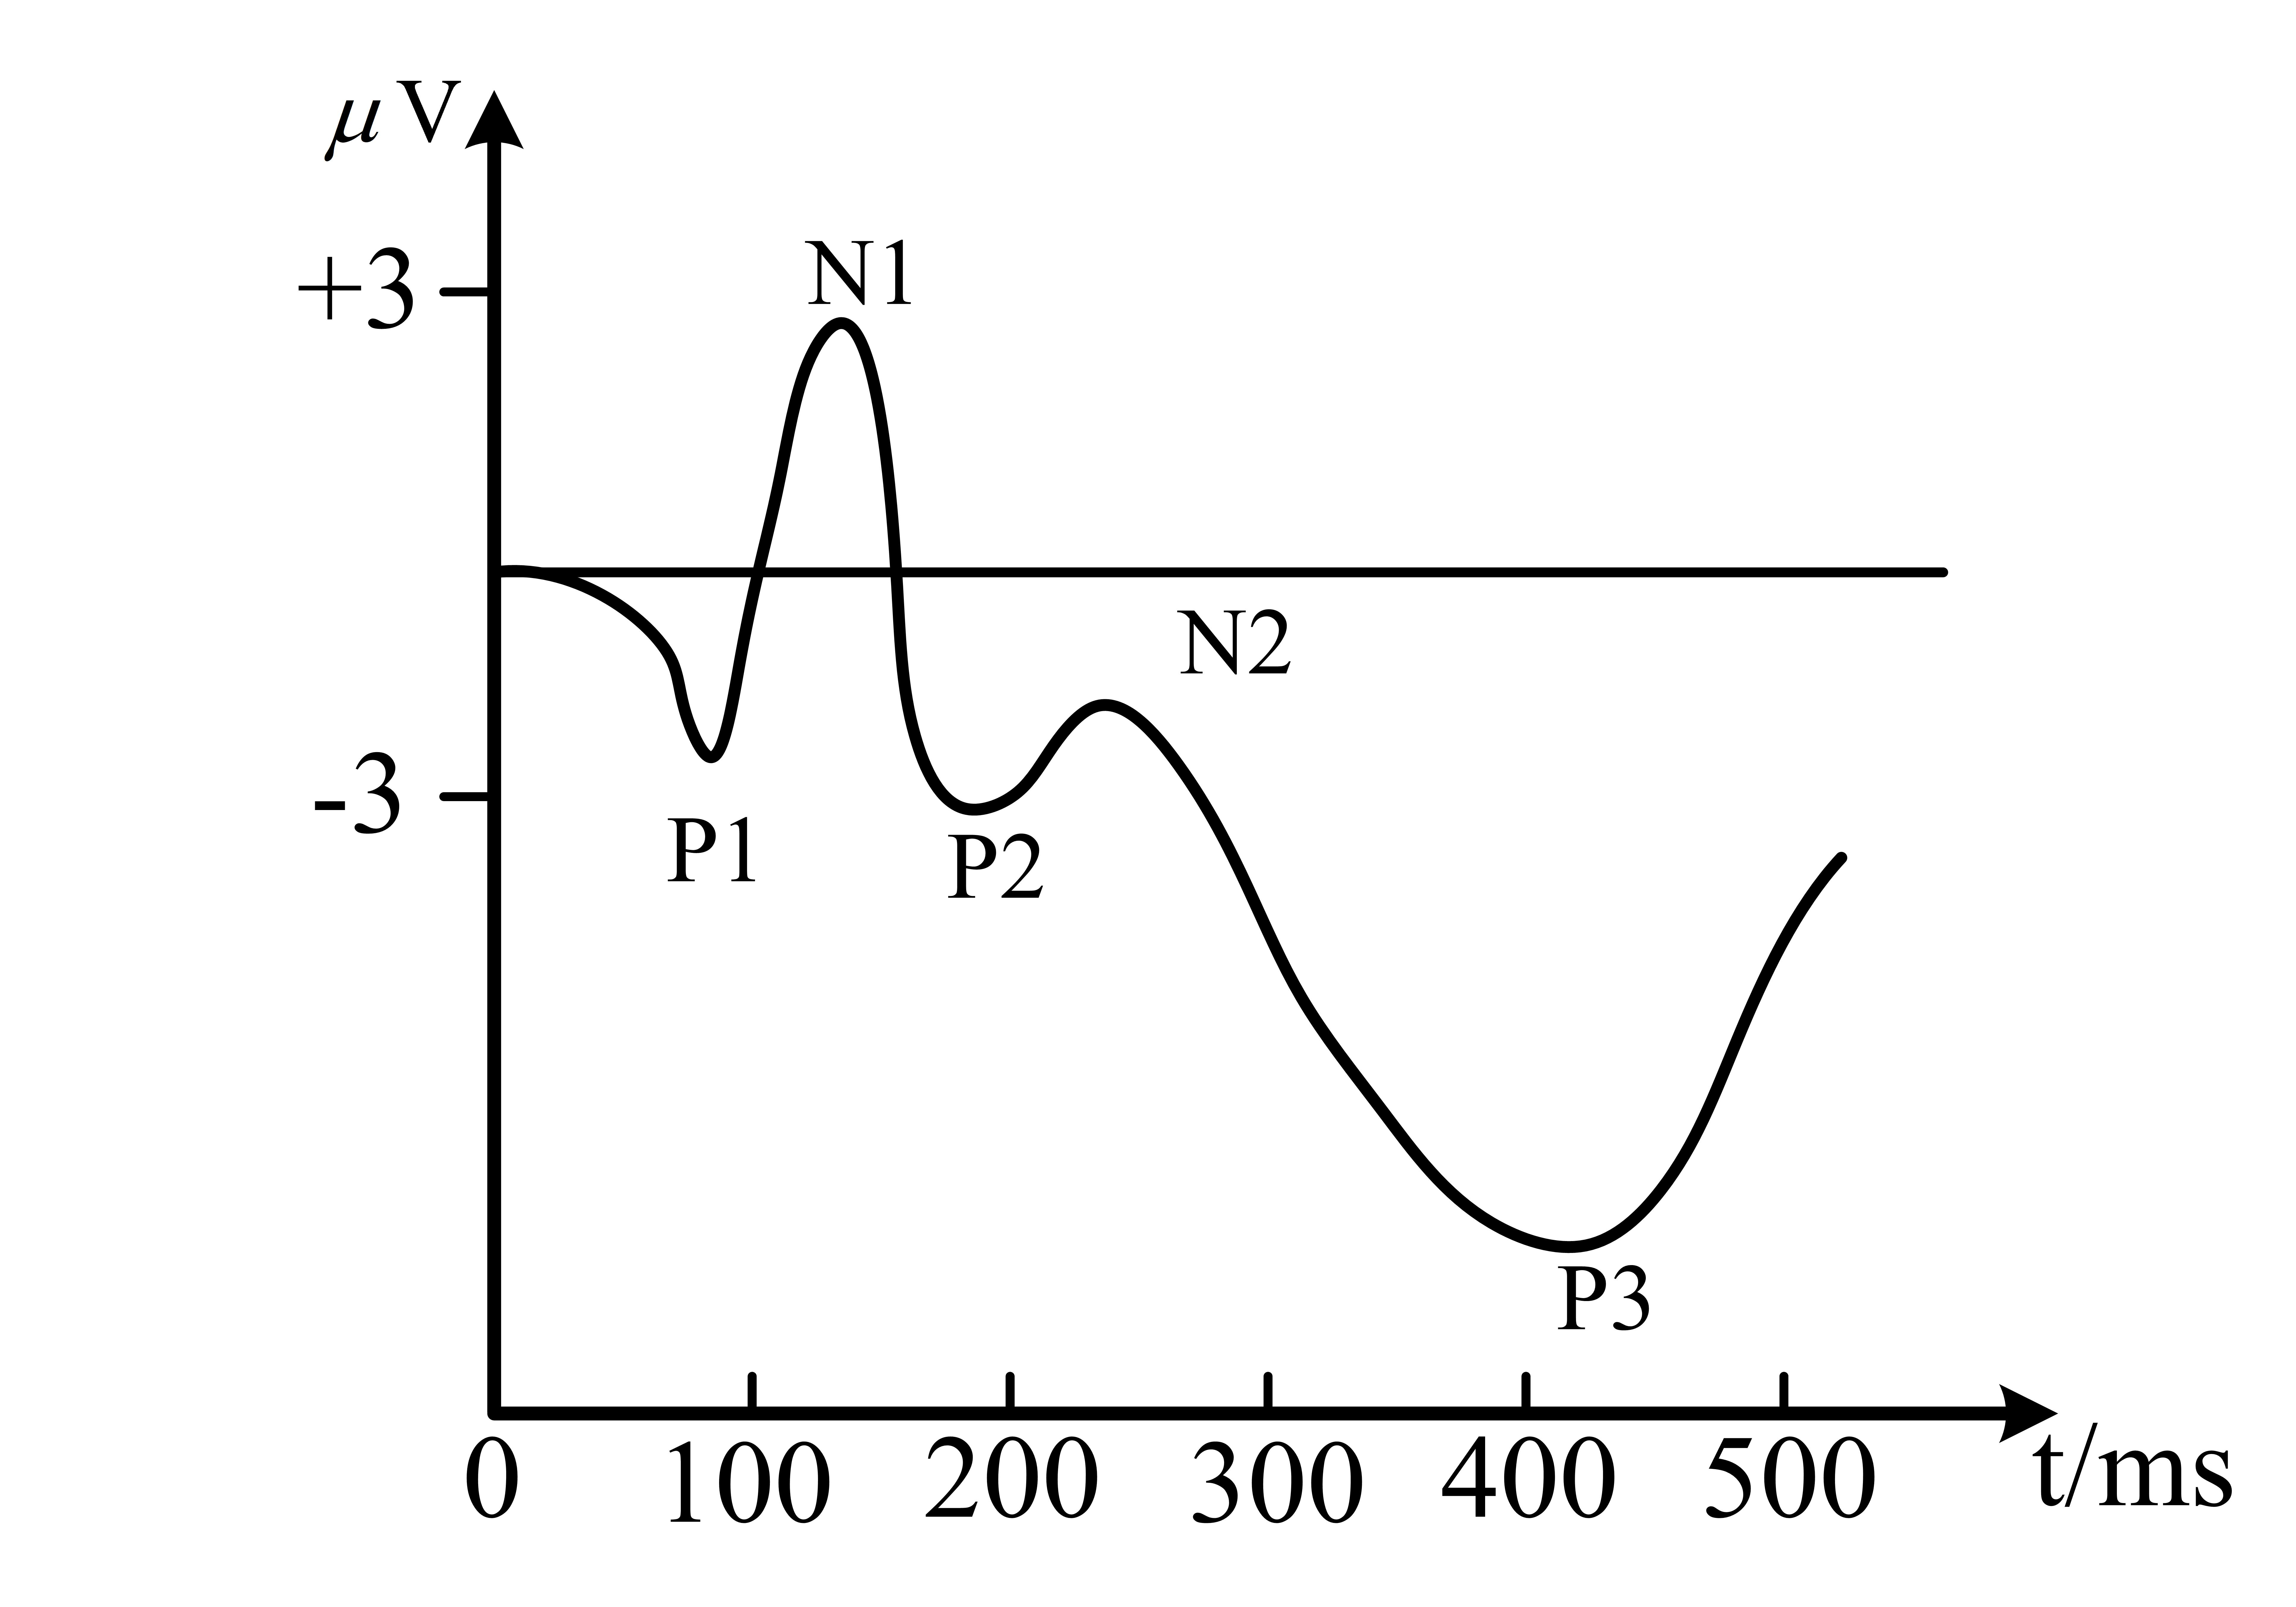
\includegraphics[width=0.3\textheight]{ERP.jpg}
	\caption{ERP相应特征}
	\label{fig1-4}
\end{figure}

(3) 基于MI范式的BCI系统

MI是人脑想象部分肢体的运动行为,而不真正执行相关动作的EEG范式。先前的研究已经证实,MI同样会激活大脑中负责产生实际动作的区域\cite{1-43}。MI在已有研究中被分类为感觉运动节律(SensoriMotor Rhythm,SMR)和想象身体运动(Imagined Body Kinematics,IBK)两类子范式。其中IBK需要使用者想象某一身体部位在三维空间的连续动作而被称为自然运动想象范式,但是这也对使用者的专业性提出了极高要求,并且需要配合较高性能EEG解码算法。因此,使用更为简单可靠的SMR范式是当前基于MI的BCI系统研究的重点。在SMR范式中,使用者需要想象身体进行一种具体运动(常见包括抬起脚、举起双手以及伸出舌头等),EEG解码算法通过分辨使用的运动意图,输出具体指令。

当进行动作想象时,人脑会在$\alpha$频段和$\beta$频段产生事件相关去同步现象(Event-Related Desynchronization,ERD)——对应频段的振幅降低;当动作想象结束后,相关频段振幅回升,即产生事件相关同步现象(Event-Related Synchronization,ERS)\cite{4-22,4-23}。特别的,在国际10/20系统的脑电极分布下,C3和C4电极位置获得的EEG信号中ERD和ERS现象尤为显著——这些电极位置位于感觉运动皮层的上方。MI中的ERD和ERS现象如图\ref{fig1-5}所示。

\begin{figure}[h]
	\centering
	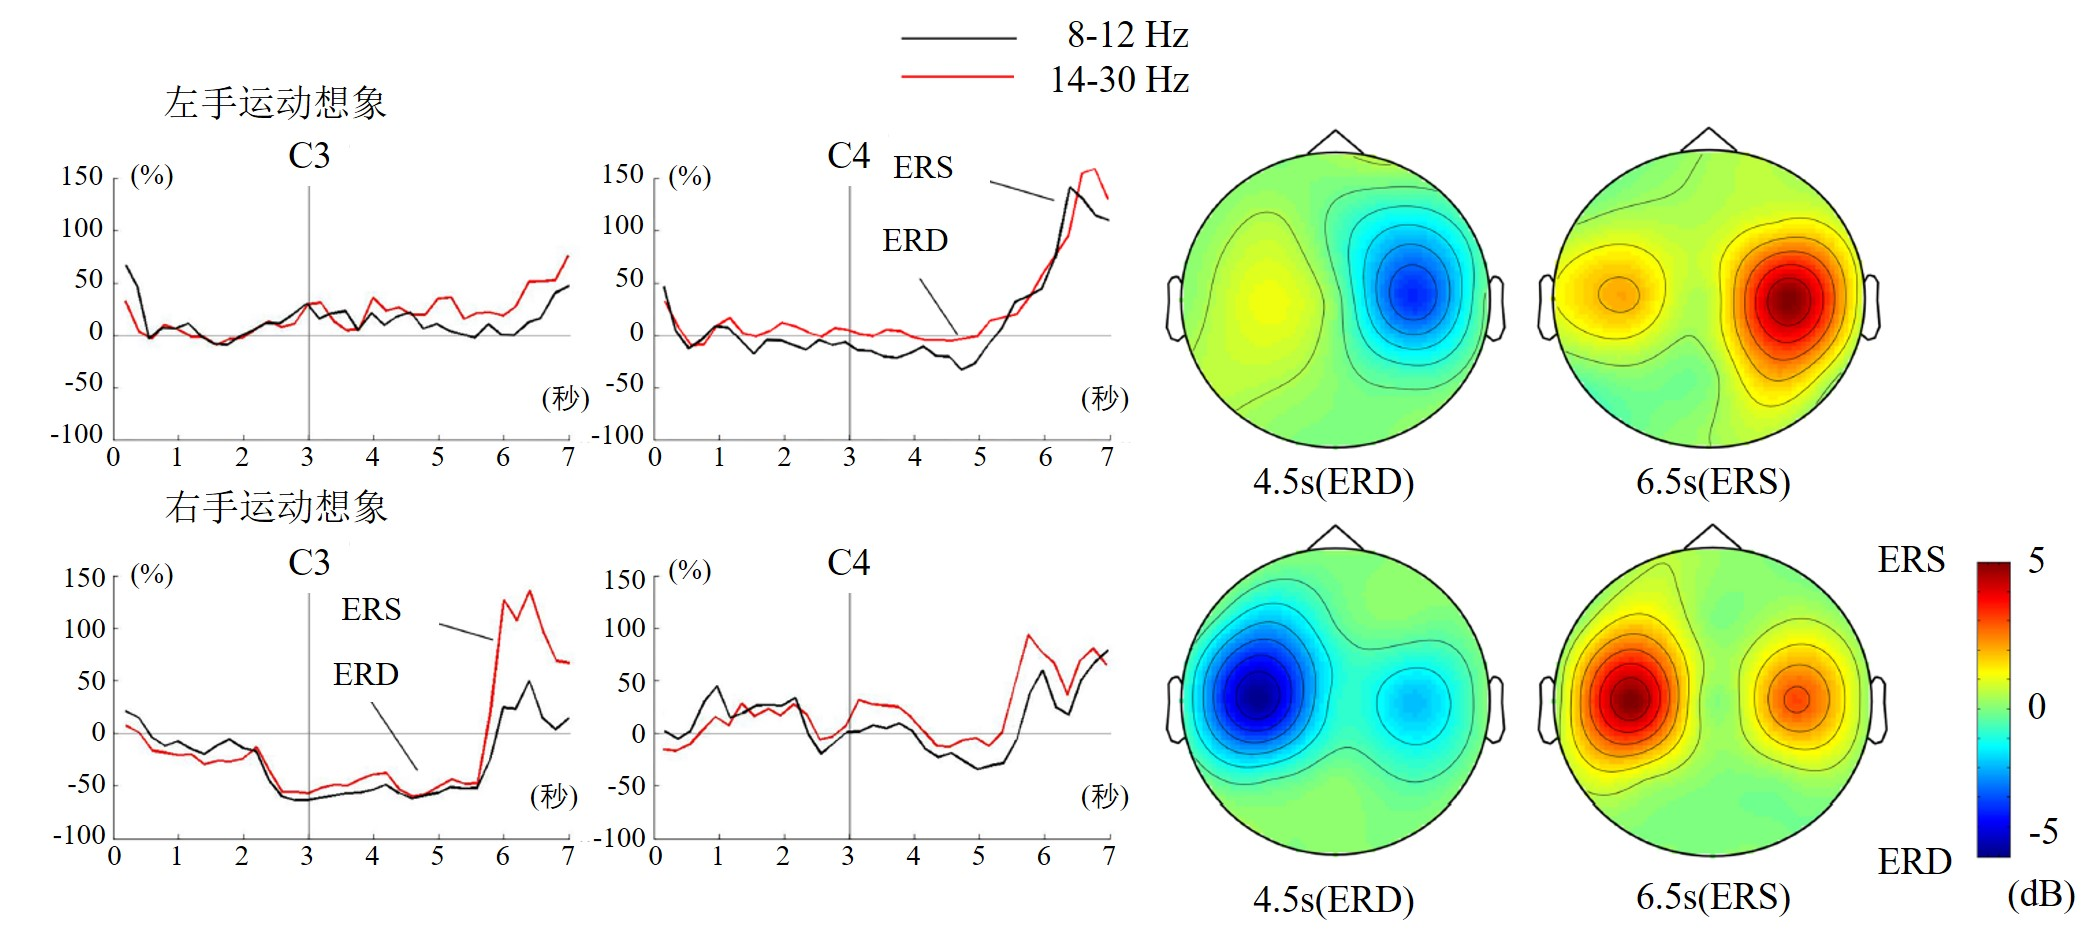
\includegraphics[width=0.60\textheight]{ERD-ERS.jpg}
	\caption{进行左右手MI任务时的ERD/ERS现象\cite{1-99}}
	\label{fig1-5}
\end{figure}

基于MI的BCI范式通过ERD和ERS现象能够进行较高精度的运动意图辨识,充分调动人体相关部位的运动神经。基于这一特点,MI在身体运动机能受损的康复治疗过程中具备极高的潜力,特别是在脑卒中患者康复领域\cite{1-44,1-45}。脑卒中患者由于脑部运动神经损伤而无法控制肢体正常运动,但是其大脑仍然保持了运动想象能力。同时,病人的患侧肢体运动机能仍然健全,因此可以通过重建神经映射通路重拾运动能力\cite{1-46,1-47}。近年来众多临床医学研究表明,基于MI的BCI系统在卒中后患者的康复进程中可以扮演重要角色\cite{1-48,1-102}。

(4) 基于被动范式的BCI系统

被动范式包括情景解释、情绪分类、意图辨识以及疲劳预警等无需进行外部刺激诱发的BCI范式\cite{1-36}。这类BCI范式不以控制意图解码为首要目的,而更关注于人脑当前状态辨识,目的是挖掘使用者的隐含信息来丰富人机交互进程。具体来说,精准的情绪辨识BCI可以让人机交互系统更加人性化,优化用户的使用体验。可靠的疲劳预警系统能够及时发现工作中的风险隐患,提醒相关人员停止作业,保证公民的生命财产安全。这一类型的BCI范式近年来同样得到了广泛关注\cite{3-28,3-29,3-30}。然而,与主动范式不同,被动范式的EEG信号往往不具有共通的显著时频域特征,这对EEG解码系统提出了较高的要求\cite{3-31}。如何设计具有一定泛化能力的被动范式BCI系统是当前亟需解决的难题。图\ref{fig1-6}展示了情绪分类EEG的采集过程。

\begin{figure}[h]
	\centering
	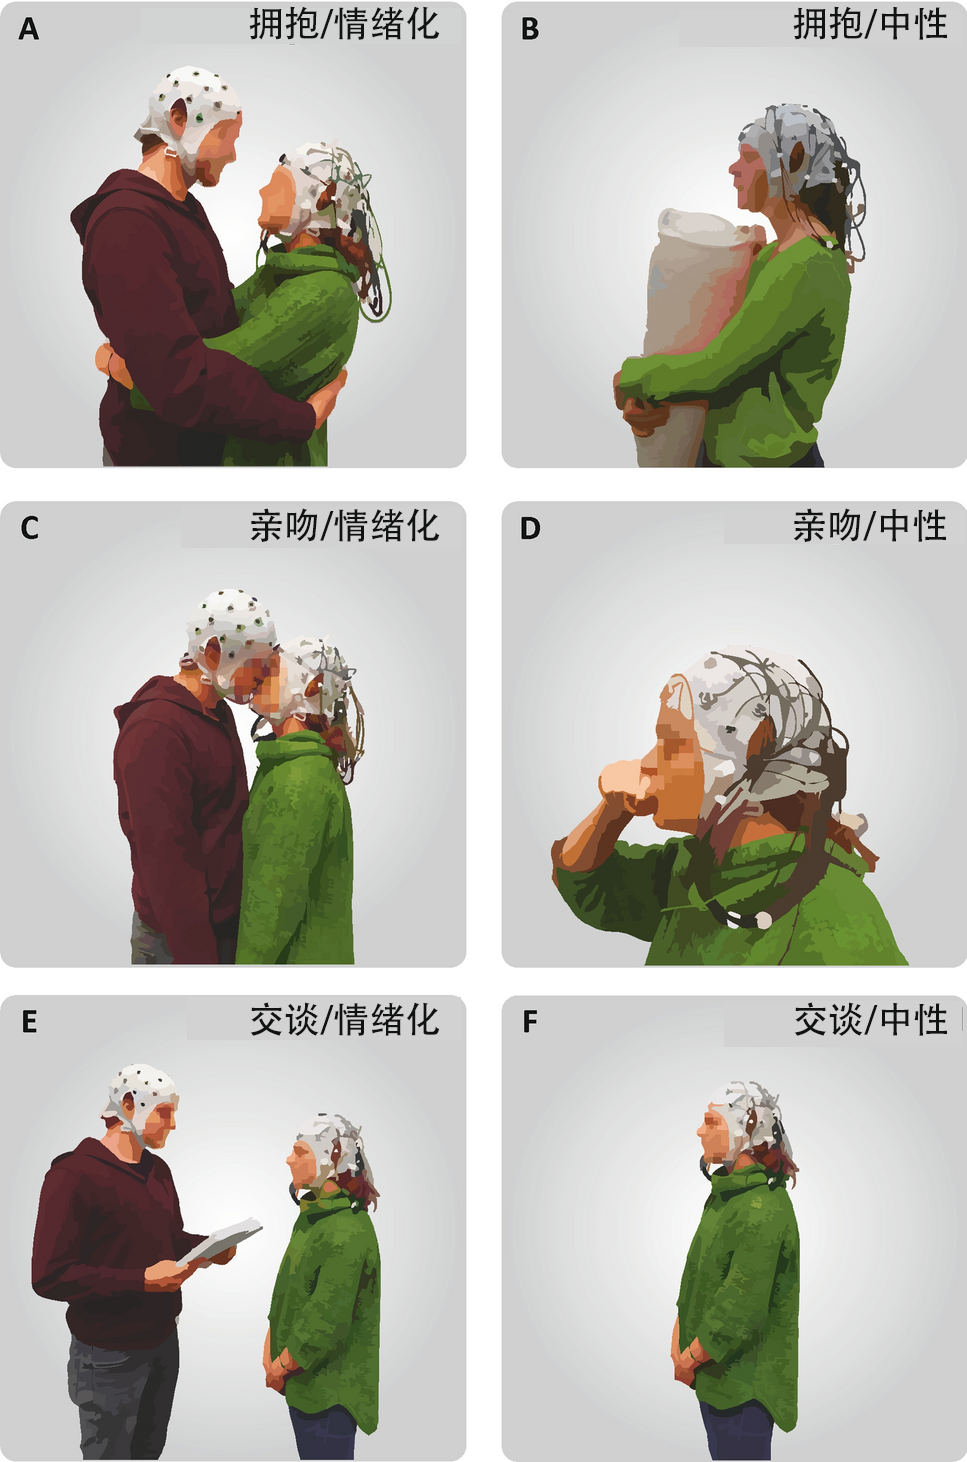
\includegraphics[width=0.3\textheight]{情绪辨识.PNG}
	\caption{情绪EEG采集\cite{1-49}}
	\label{fig1-6}
\end{figure}


不同范式的BCI系统所获取的EEG信号具有不同的分类难度,其中SSVEP和ERP范式由于其显著的时频域特点而相对容易辨识。MI范式和被动范式的EEG信号则由于其难以寻找通用性特征仍面临着分类精度不足的问题,设计合理的分类辨识模型是BCI走向实际应用的关键。


\subsection{国内外EEG采集设备}
EEG采集设备在发展过程中,逐渐分化出了侵入式\cite{1-50}与非侵入式\cite{1-51}两条不同的分支。

侵入式EEG采集设备追求可靠的信号质量,更高的信噪比以及更少的外部生理信号干扰,直接将EEG电极通过手术的方式植入使用者大脑内部。这一采集手段的EEG电极直接与大脑进行接触,使其在拥有较为纯净优质信号的同时,也为使用者带来巨大的手术风险,直接对使用者的日常生理活动造成负面影响。因此,基于侵入式的EEG 采集设备在医疗科研领域拥有广阔前景\cite{1-52},但其并没有在现实生产生活中得到推广\cite{1-53}。图\ref{fig1-7}展示了侵入式脑电极在大脑中的排布方式。

\begin{figure}[h]
	\centering
	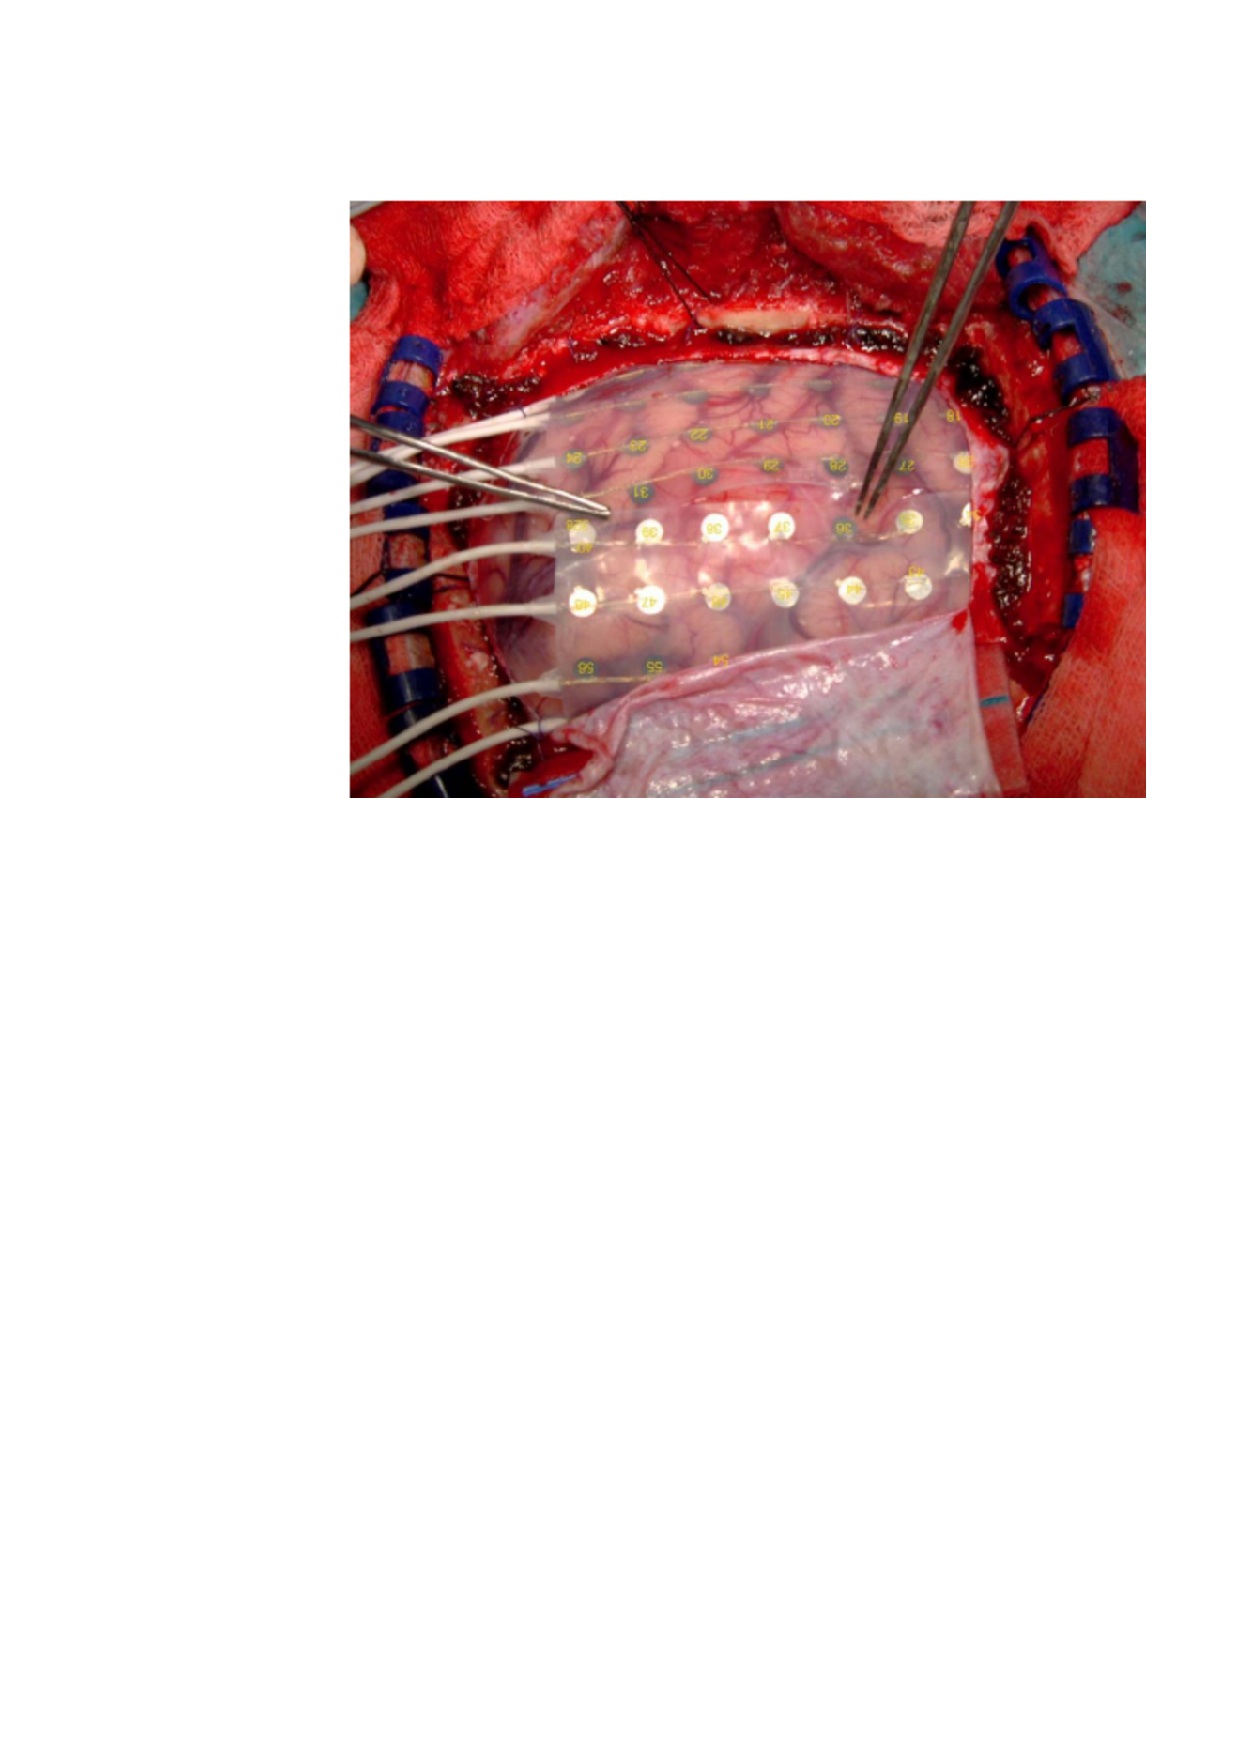
\includegraphics[width=0.33\textheight]{侵入式.pdf}
	\caption{侵入式EEG电极排布\cite{1-54}}
	\label{fig1-7}
\end{figure}


非侵入式EEG采集设备通过安置在大脑皮层外侧的脑电极进行获取,这些电极通常嵌入在脑电极帽中。这种采集手段的目的在于追求实用性,因为其无需进行手术,电极安装过程较为简便,没有过高的使用门槛,成本远低于侵入式设备。非侵入式EEG采集设备保留了高时间与空间分辨率的优点,并且其信号信噪比仍处于可接受的范围,因此在近年来得到了广泛关注\cite{1-55}。本文的工作即基于非侵入式EEG采集设备展开。

\begin{figure}[h]
	\centering
	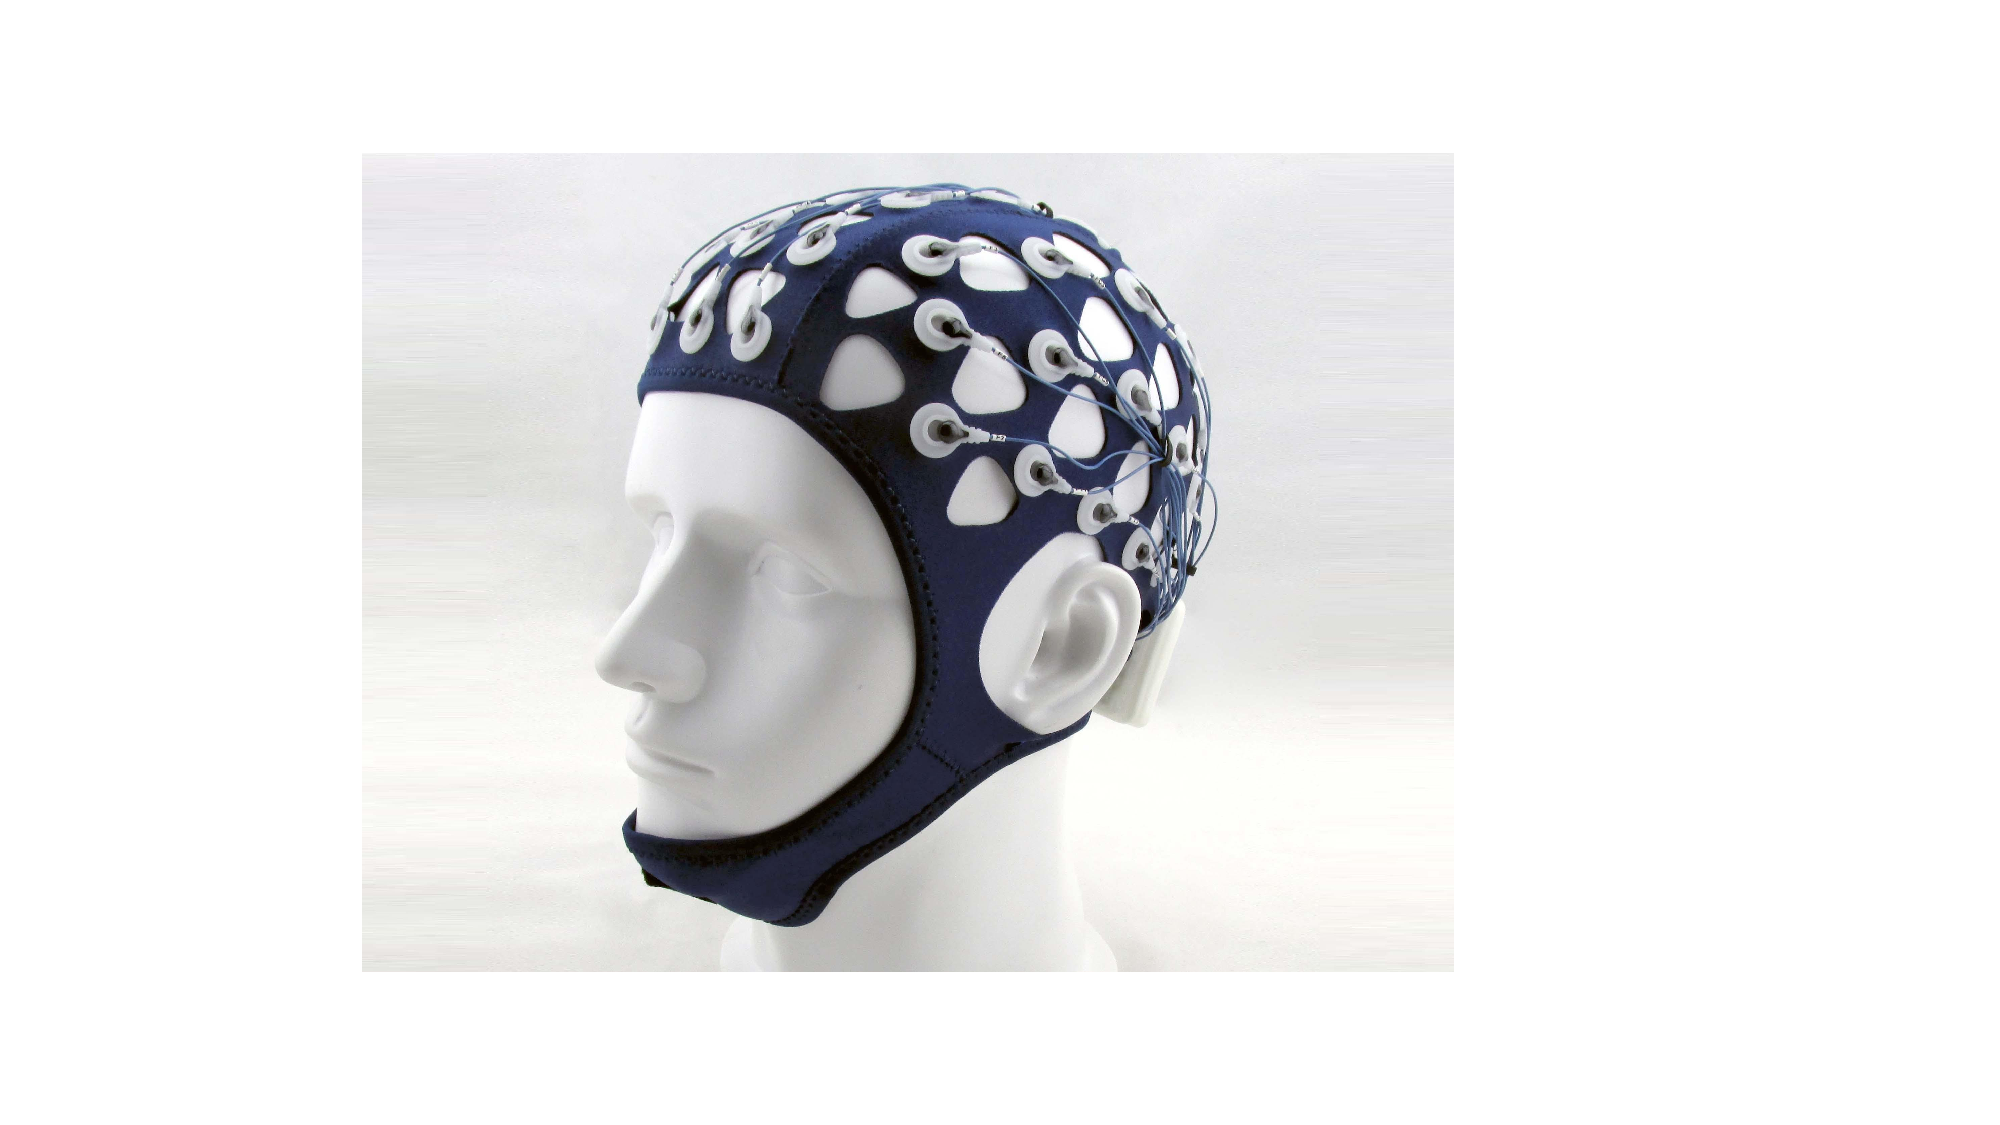
\includegraphics[width=0.33\textheight]{非侵入式.pdf}
	\caption{非侵入式EEG电极排布}
	\label{fig:graph3}
\end{figure}

当前国内外EEG采集设备已经具备了一定的成熟度,其中国外EEG研究起步较早,因此发展速度较快,产品种类较多。具有代表性的包括Neuroscan公司的Neuroscan Amplifiers系列产品、EGI公司的GTEN-200系列产品、Emotiv公司的便携式人机交互系统等。Neuroscan Amplifiers系列作为研发最早的EEG采集设备之一,已经发展出了十余种性能优异的不同采集子系统。其产品覆盖面较广,拥有29通道、32通道、64通道以及256通道等多种应对不同需求的EEG采集设备。其中常见的SynAmps RT 64-channel Amplifier设备能够以20000 Hz同时采集64通道EEG信号,每个通道包括一个24位的A/D转换器。这个采集系统除了用于EEG采集的导联盒和脑电极帽以外,还包括专用的电源盒(Power Unit)和控制盒(System Unit)。SynAmps RT 64-channel Amplifier系统的整体重量在10 kg以上,售价超过10万元,且体积较为庞大。EGI公司的GTEN-200系列产品能够采集32-256通道的EEG数据,其配套有先进的成像软件,能够绘制逼真的高分辨率人脑模型,是当今最先进的非侵入性神经调节系统之一。GTEN-200系列的64通道产品整体售价超过50万元,并且系统较为庞大,操作流程复杂。与前两种主要面向医疗科研领域的产品不同,Emotiv公司的便携式人机交互系统面向普通人的日常生活场景。其使用16通道的干电极采集EEG信号,并通过蓝牙对外设进行控制。它的设计理念更倾向于便携与日常使用,因此采集信号的质量较差。国内neuracle公司的EEG采集设备也已经得到了相关领域的认可,其设计生产的系列产品同样具备优异的采集性能与人脑状态辨识能力。

通过上述介绍可以看到,高精度的多通道EEG采集设备往往体积庞大,操作环节复杂,价格极高,仅能面向医疗科研使用。消费级的EEG采集设备存在着通道数较少,信号质量不佳的问题。因此,设计开发一款体积较小,通道数量较多,价格亲民的EEG采集设备对BCI系统的落地与推广具有一定的现实意义。本文将遵循这一思路,设计基于EEG的BCI系统,并对采集得到的EEG信号进行辨识分析。

\section{基于深度学习技术的脑电信号分析}
为了真正意义上实现BCI系统的广泛应用,BCI系统所收集的EEG信号能否被准确辨识已成为当前BCI性能评估的一个重要指标。针对不同的EEG范式,相关研究人员提出了众多特征提取方法,比如傅里叶变换(Fourier Transform)、表面-拉普拉斯变换(Surface-Laplacian Transform)、共空间模式(Common Spatial Patterns,CSP)以及基于熵的分析方法\cite{1-56, 1-57, 1-58, 3-11}。这些特征与支持向量机(Support Vector Machine,SVM)、近邻分类器(Nearest Neighbor Classifiers)以及逻辑回归(Logistic Regression)等传统机器学习分类器的结合为BCI系统的实现做出了巨大贡献\cite{1-59,1-60,1-61}。然而,基于这一设计思路的模型较为依赖于设计者的专业知识,缺乏足够的泛化性能。提升模型泛化性能的直观方法是增加通用信息的权重,并通过精确选择与任务相关的EEG通道来提高分类性能\cite{1-62}。此外,直接寻找关键性特征将为BCI系统带来更多的性能收益\cite{1-63}。

深度学习技术在过去十年中发展迅速,在图像处理和复杂时间序列分析中表现出强大的分类和辨识能力\cite{1-64}。经典的深度学习模型包括多层感知机(MultiLayer Perceptron, MLP)\cite{1-68}、循环神经网络(Recurrent Neural Networks, RNN)\cite{1-69}、玻尔兹曼机(Deep Boltzmann Machines, DBM)\cite{1-70}和卷积神经网络(Convolutional Neural Networks, CNN)\cite{3-21}等,其典型结构如图\ref{fig1-8}所示:

\begin{figure}[!h]
	\centering
	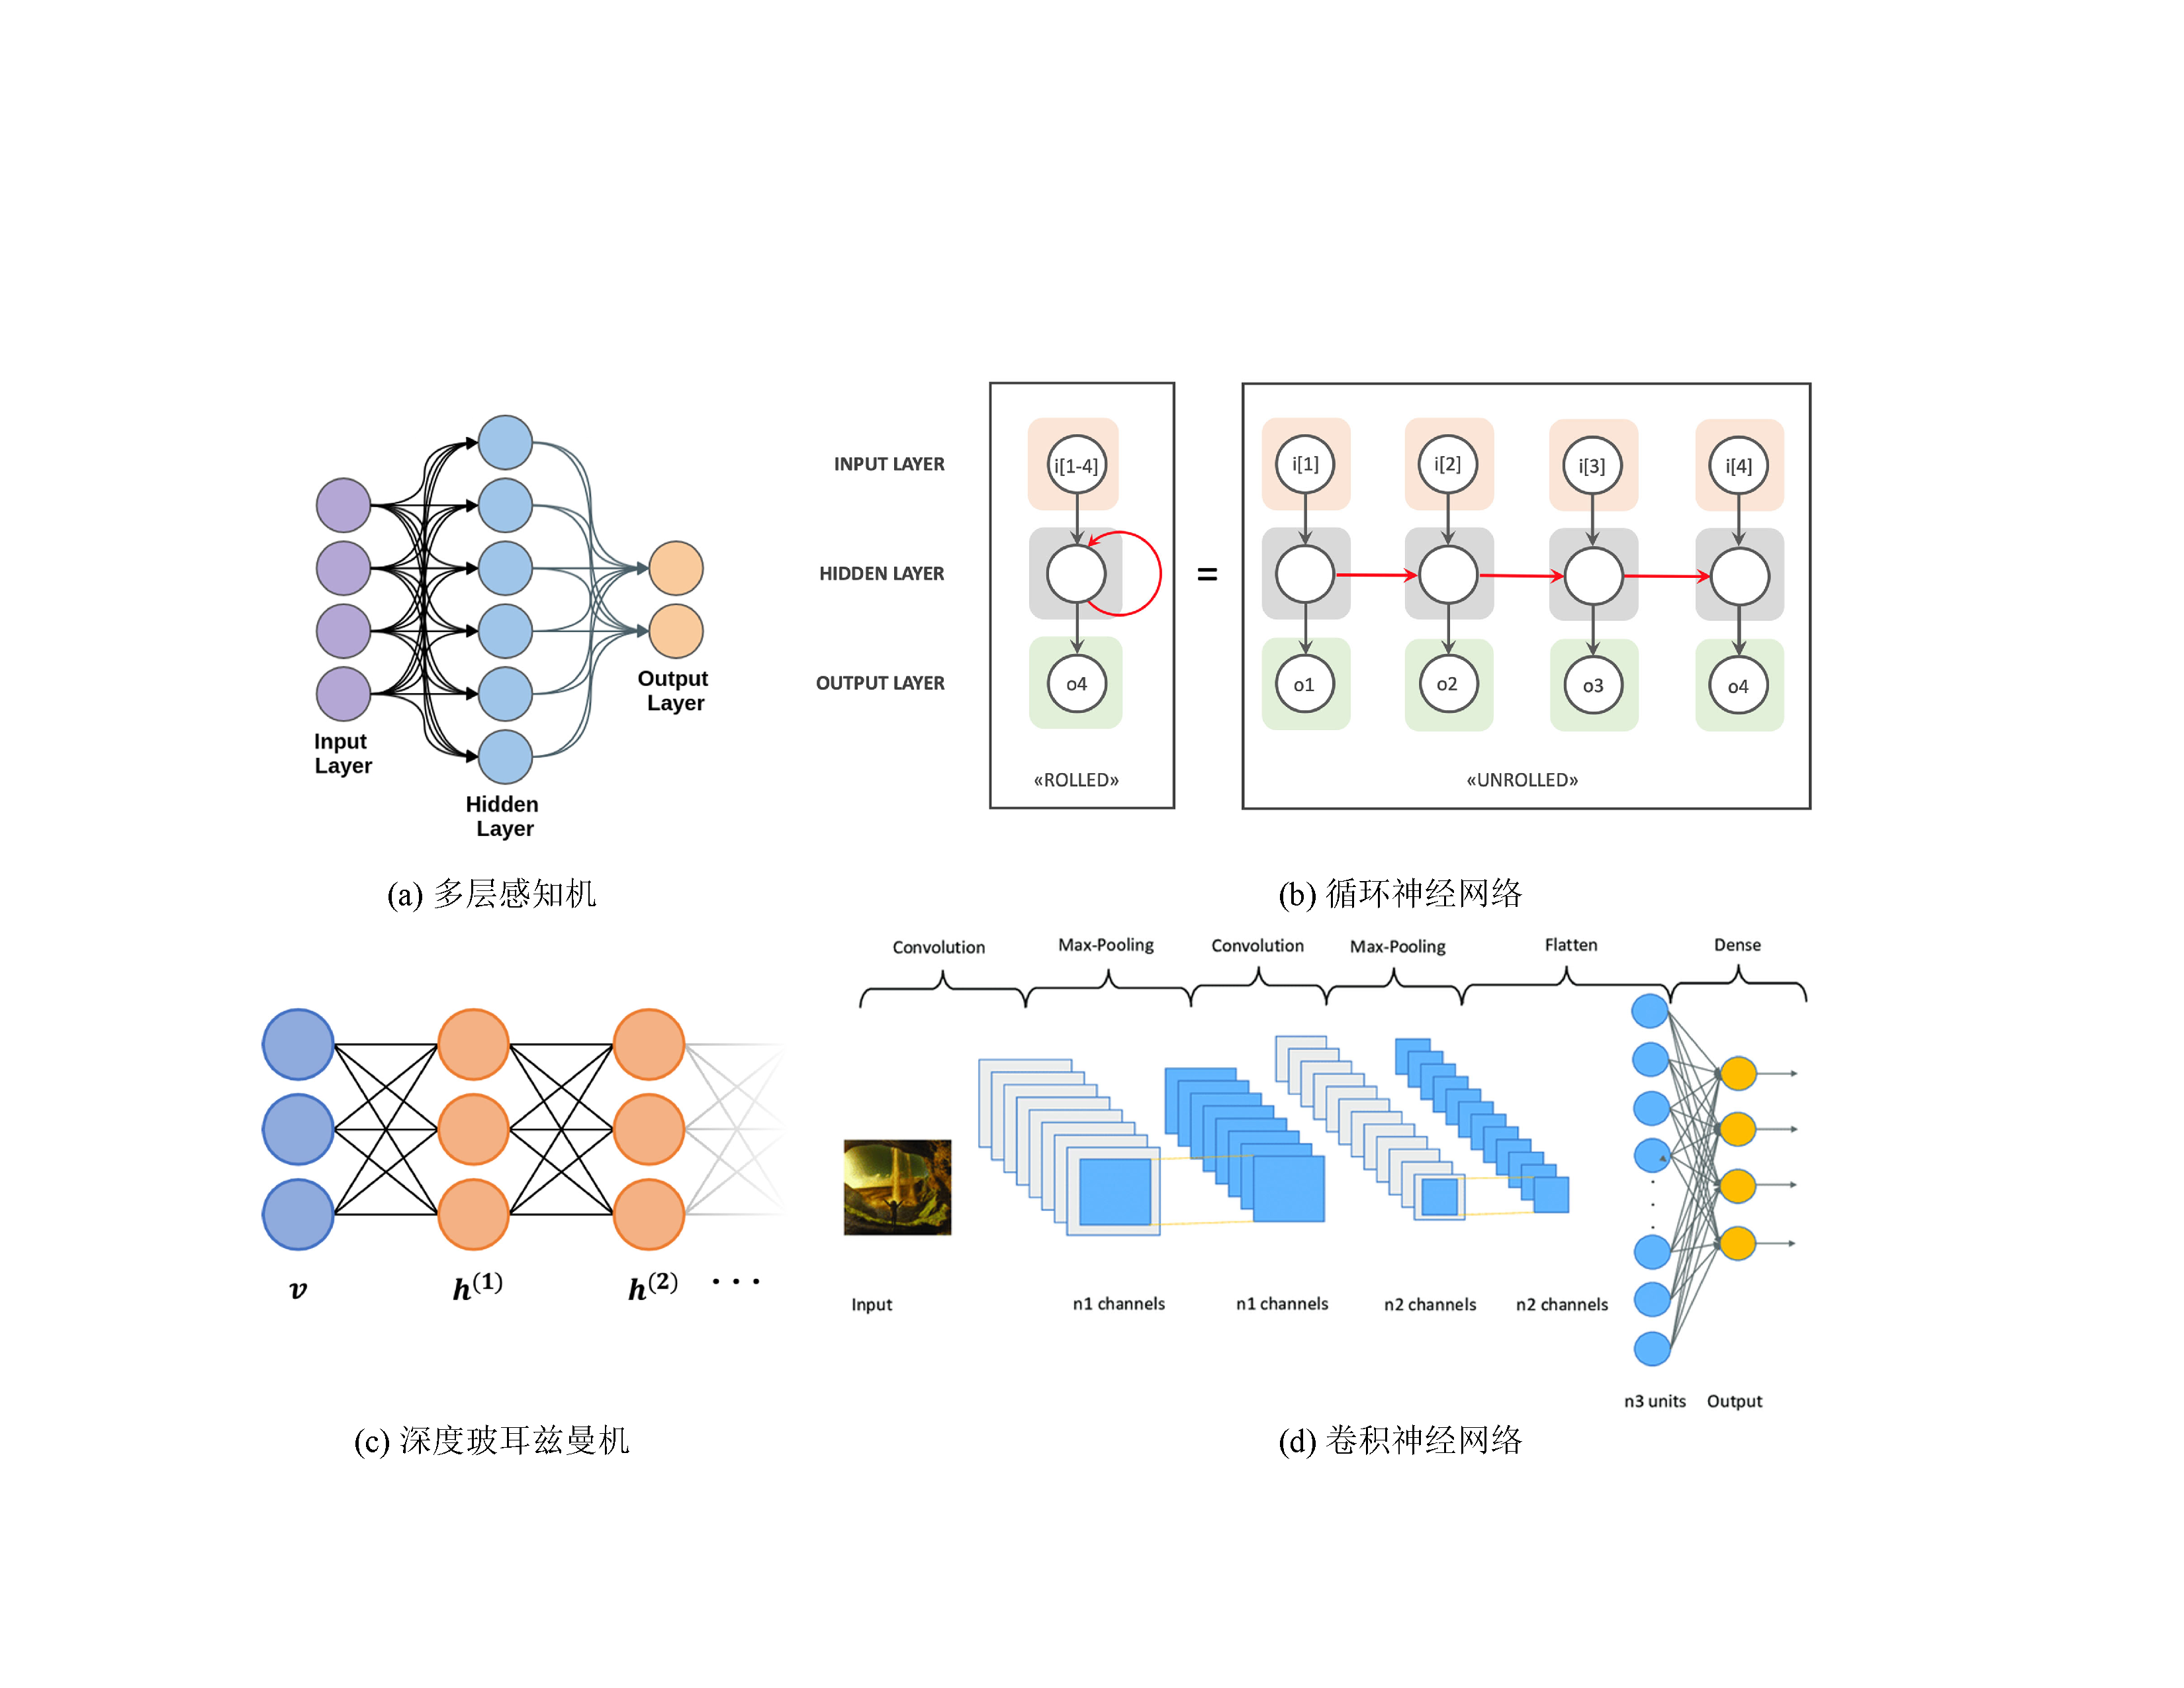
\includegraphics[width=0.60\textheight]{DL.pdf}
	\caption{深度学习模型典型结构}
	\label{fig1-8}
\end{figure}

深度学习模型具备的数据驱动和强大的特征提取能力,使其能够从大量的EEG信号中挖掘通用特征,减轻模型设计对于专家知识的依赖性。无论是基于主动范式SSVEP,ERP以及MI的EEG信号,抑或是基于被动范式情绪,疲劳以及脑负荷的EEG信号,深度学习均在其上取得了极具竞争力的结果\cite{1-66,1-67}。Gao等人\cite{1-65}基于EEG信号的时空特性,针对性的改造了卷积神经网络,引入具有时间和空间属性的卷积模块,在基于EEG的疲劳辨识任务中取得了极高的准确率。Xu等人\cite{1-71}在循环生成对抗网络(Cycle-consistent Adversarial Networks,CycleGAN)的基础上,保留EEG信号的频域特征与空间信息,生成脑卒中患者的EEG数据以扩展训练数据样本数量,实现对卒中患者运动意图的有效辨识。Ma等人\cite{1-72}成功地融合了深度置信网络(Deep Belief Network,DBN)和压缩感知技术,有效降低了DBN的训练复杂度,并将其成功应用于EEG分类。Tsiouris等人\cite{1-73}利用预训练策略,寻找LSTM模型种各模块的最优结构,之后构建两层LSTM网络对基于EEG的癫痫发病情况进行预测,为癫痫疾病的治疗提供辅助。He等人\cite{1-74}基于图注意力网络(Graph Attention Networks)和双向LSTM挖掘癫痫EEG数据的时域特征,并根据当前时刻的前后状态做出最终决策。结果表明,这一模型能够在两种常见的公开数据集上取得当下最优的结果。Khademi等人\cite{1-75}设计了一种混合结构的端到端MI范式EEG信号分类模型。其同时搭建三种不同的模型结构以应对单一模型可能出现的梯度消失或者表征能力不足问题,并使用迁移学习和数据增强算法提升模型的泛化性能。最终的结果表明,其拥有当下最具竞争力的MI辨识性能。

\section{神经架构搜索技术的发展及其与脑电信号辨识研究的融合}
尽管基于深度学习的EEG研究已经取得了瞩目的成果,但是这些方法也继承了深度学习模型结构设计困难、需要专业的设计经验与先验知识、依赖长时间的人工调试和优化等问题,阻碍了BCI系统的实现和普及。针对上述问题,神经结构搜索(Neural Architecture Search,NAS)概念应运而生\cite{1-76}。遗传算法\cite{1-77}、强化学习\cite{3-33}和贝叶斯优化算法\cite{1-78}已被成功应用于NAS进程中,这些方法在一定程度上解决了网络架构设计的问题,使模型根据数据信息自动获取合适的网络架构成为可能。

基于某种搜索策略,依靠预定义的候选操作集和搜索空间来探寻不同网络架构带来的性能变化,是NAS算法的设计策略。通过对生成的子网络的性能进行排序,并反馈不同架构带来的性能变化,搜索策略被不断优化。当得到的子网络满足网络性能要求时,搜索过程就会停止,并得到当前条件下的最佳网络架构\cite{1-76}。举例来说,基于神经网络的内部结构可以被编码为可变长度字符串的特性,利用强化学习能够生成最佳网络架构\cite{1-79}。Baker等人\cite{1-80}提出了“Meta-QNN”,它创新性地将网络架构搜索建模为马尔可夫决策过程,并使用强化学习中的Q-learning算法来寻找最佳CNN架构。为了提高计算速度,Zoph等人\cite{1-81}提出了“NASNet ”搜索模型,即先在一个小数据集上搜索网络结构,然后再迁移到一个大数据集上,从而减少结构搜索过程中的资源消耗,这一搜索策略被命名为代理搜索。Bender等人\cite{1-88}在已用NAS算法的基础上,创新性地将CNN架构设计为多个“Cell”结构的堆叠,而“Cell”结构被看作是一个包含N个有序节点的有向无环图。这一名为“one-shot”的结构设计,成为了后续NAS算法的基础。图\ref{fig1-9}展示了经典的“one-shot”搜索框架。

\begin{figure}[!h]
	\centering
	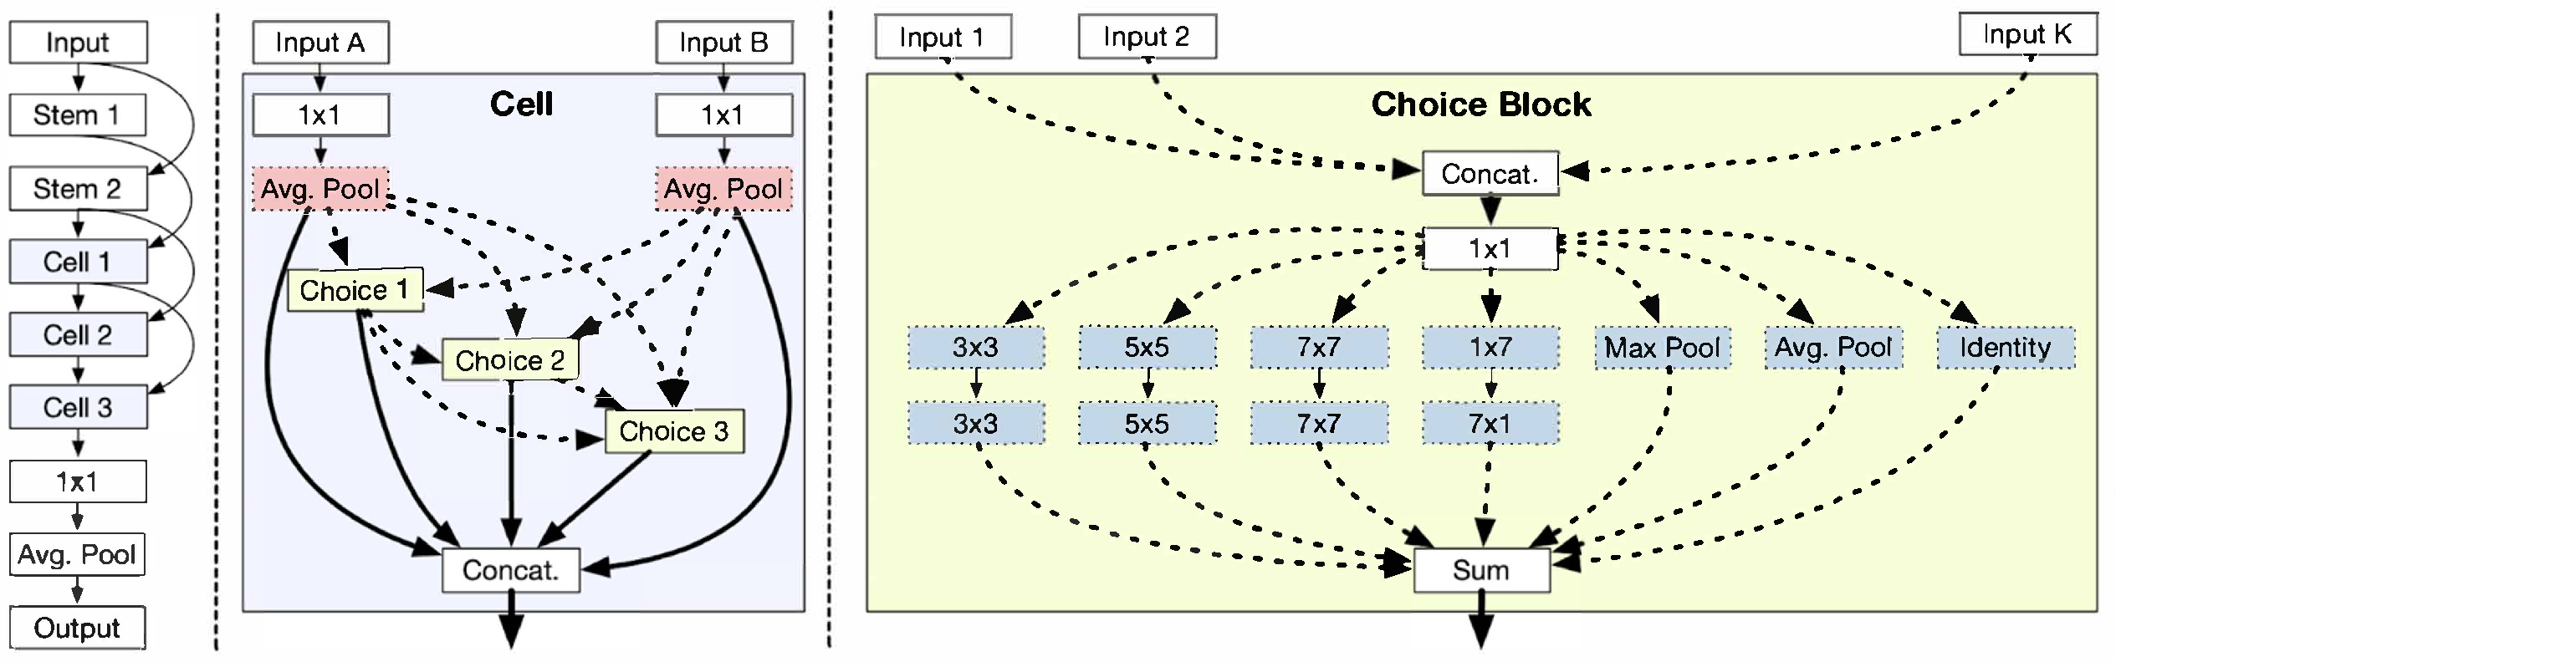
\includegraphics[width=0.60\textheight]{NAS.pdf}
	\caption{“one-shot”搜索框架\cite{1-88}}
	\label{fig1-9}
\end{figure}

然而,上述方法并没有改变NAS过程作为一个“黑箱”的本质,为了解决这个问题,基于梯度的NAS算法被开发出来。DARTS\cite{3-34}算法遵循Bender等人\cite{1-88}的设计,在“one-shot”搜索框架的基础上将梯度引入模型结构搜索中。基于梯度的算法同时优化了模型的结构权重和层权重,有效减少了结构搜索的时间和性能消耗。为了进一步减少内存占用,在DARTS的基础上,P-DARTS\cite{1-82}和PC-DARTS\cite{3-7}被研发出来,并取得了巨大的成功。PC-DARTS的成功不仅取决于其创新的部分通道搜索算法,而且还取决于其继承的DARTS搜索空间。DARTS的模块化搜索结构,连续的搜索空间合理降维了庞大的搜索区域,进一步提升了搜索效率。图\ref{fig1-10}展示了PC-DARTS的搜索流程。

\begin{figure}[!h]
	\centering
	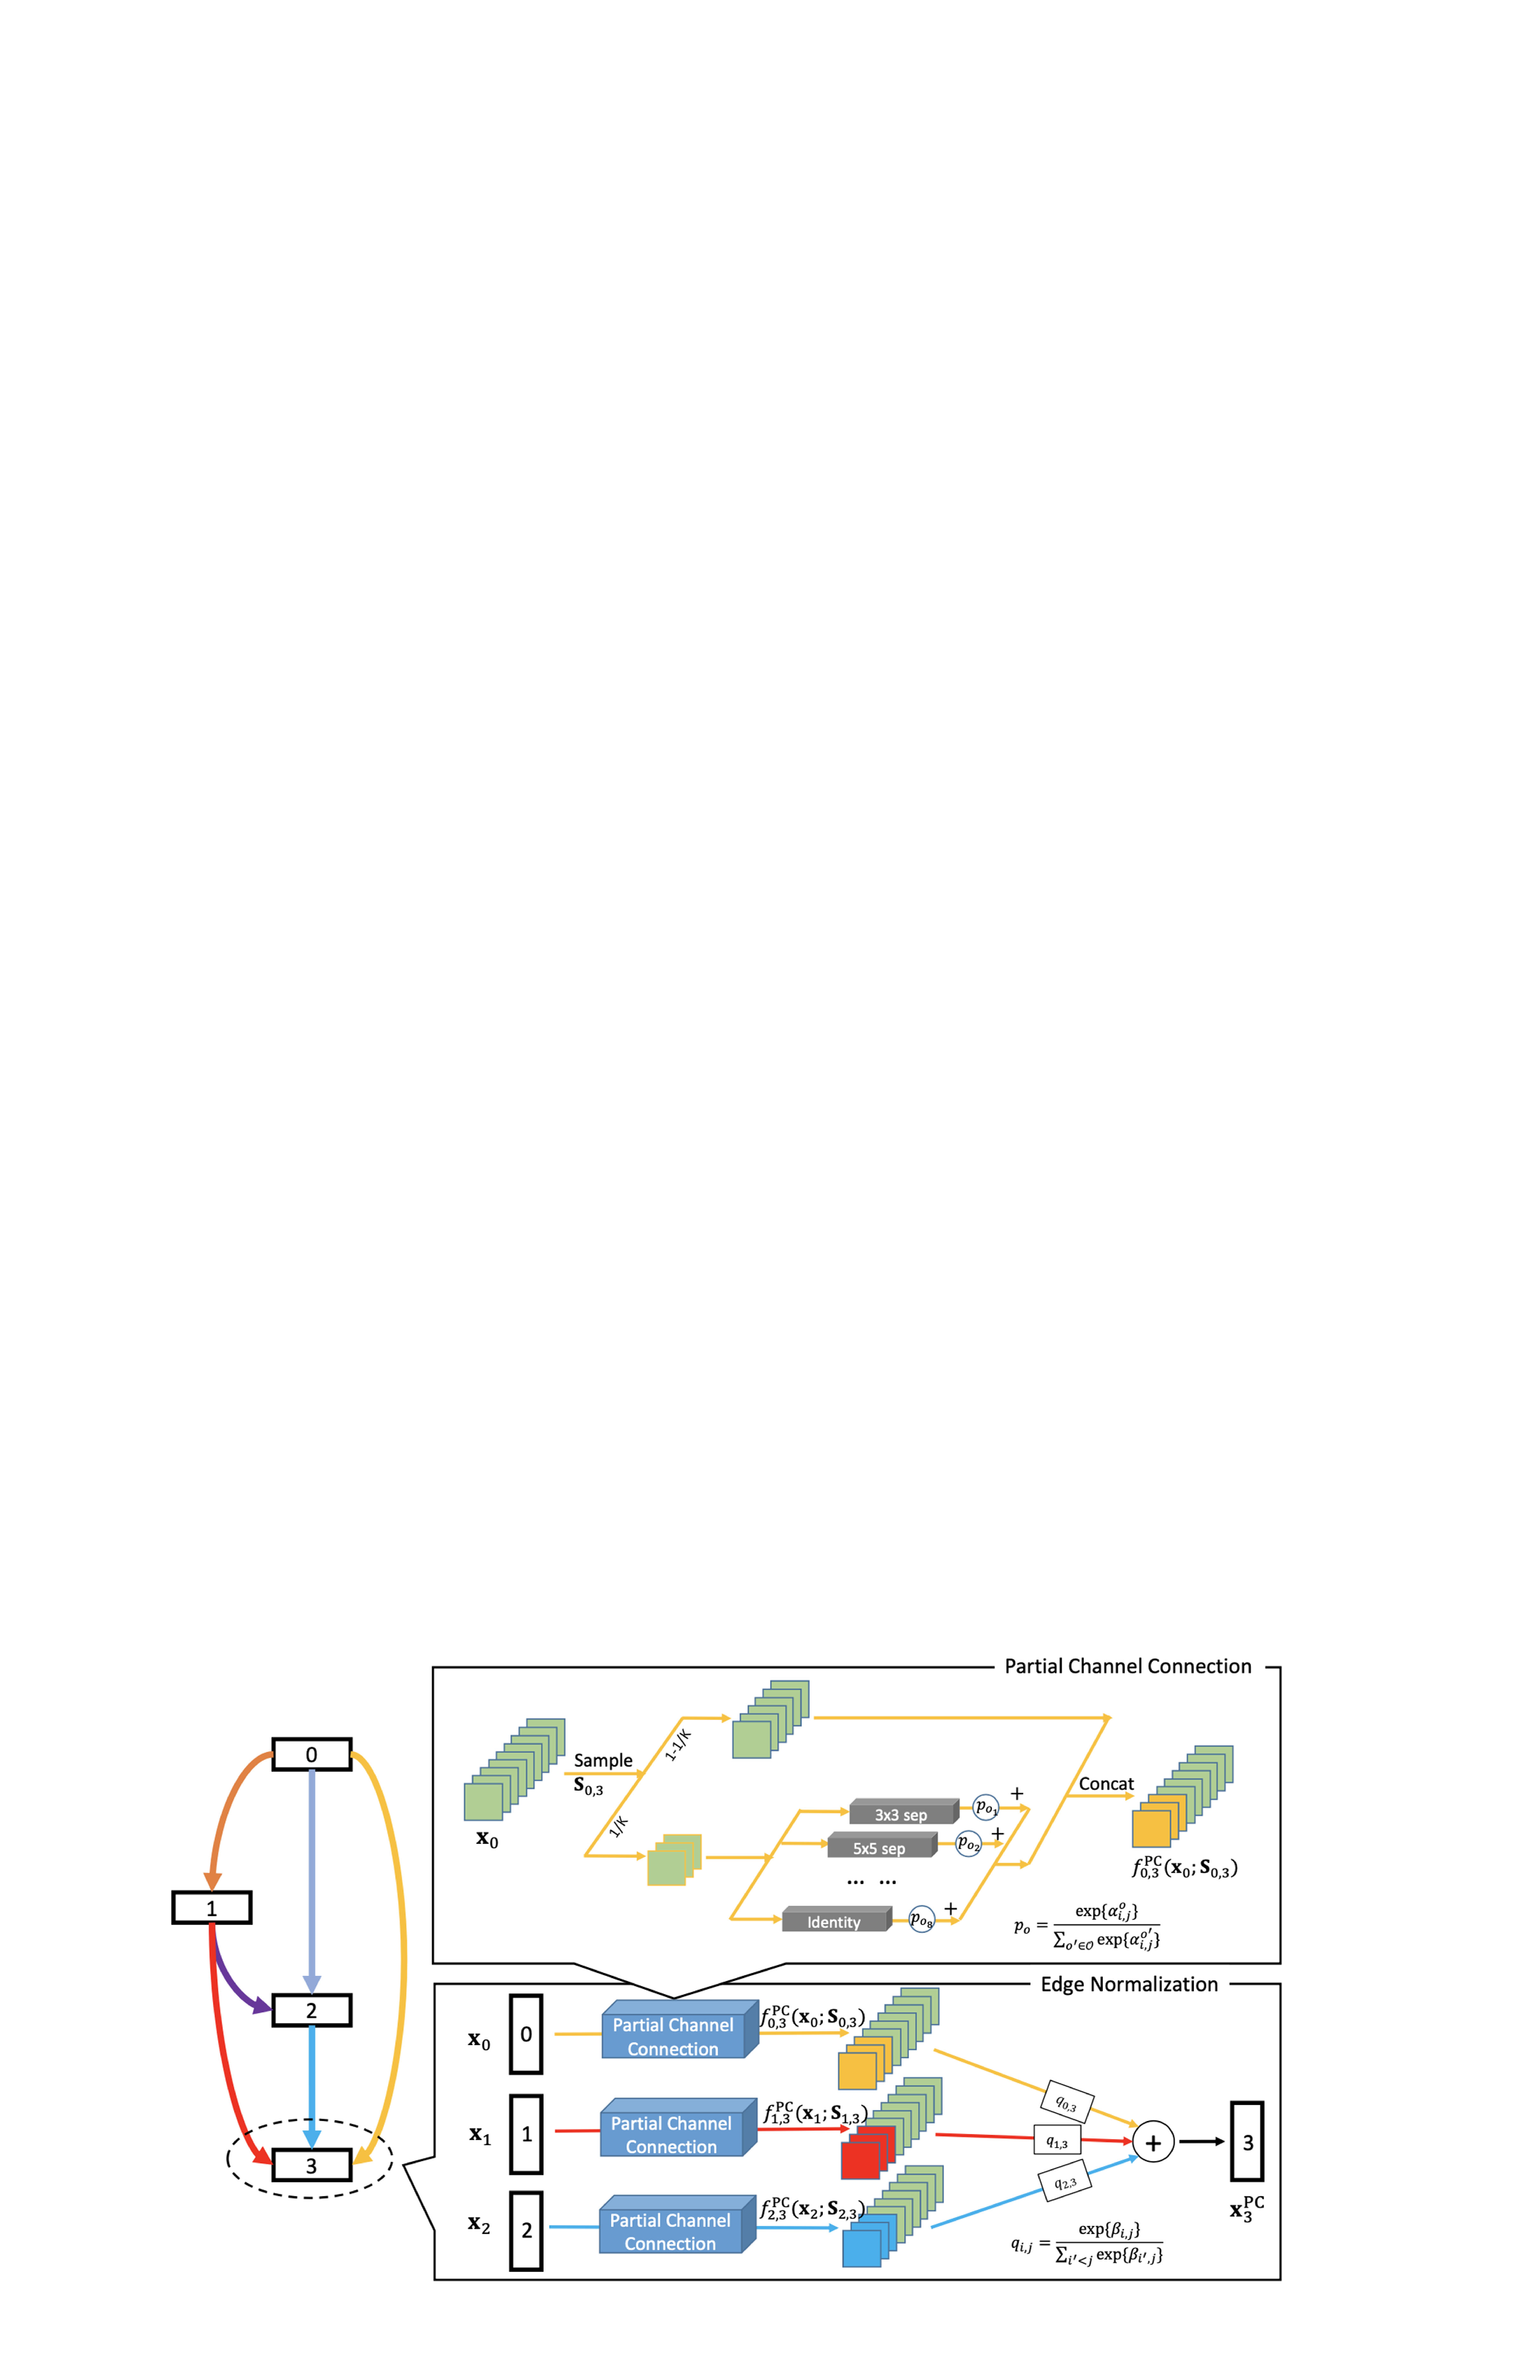
\includegraphics[width=0.52\textheight]{PC-DARTS.pdf}
	\caption{PC-DARTS算法流程\cite{3-7}}
	\label{fig1-10}
\end{figure}

基于EEG的NAS技术在近年来得到了一定关注。Li等人\cite{1-83}遵循基于强化学习的NAS\cite{1-79}设计思路,使用RNN作为控制器生成网络结构,并使用强化学习训练控制器使其逐步降低模型分类损失。其最终结果在两款情绪EEG的公开数据集上优于人工设计的CNN模型。Li等人\cite{1-84}将NAS策略与Transformer模型相结合,在NAS进程中兼顾模型的最终精度和空间复杂度,得到极具竞争力的情绪EEG辨识模型。Du等人\cite{1-85}利用多目标进化算法实现针对SSVEP范式EEG信号的NAS进程,并对生成的子网络应用网络模态(Network Morphism)和贝叶斯优化技术,以获取性能最优的搜索结果。Xue等人\cite{1-86}同样引入基于遗传算法的NAS模型,充分利用了遗传算法的启发式搜索和不需要梯度的优势来搜寻最优CNN架构。其结果证明,搜索得到的CNN模型能够在基于EEG的睡眠阶段分类任务中战胜当前最优算法。

从上述结果可知,尽管基于梯度的NAS模型具有相较于其他NAS算法更高的可解释性和更小的计算资源消耗,但是现有研究还并未将其迁移至EEG分类辨识领域。同时,现有算法针对单一范式EEG数据进行搭建,其泛化能力仍然存在提升空间。

\section{无监督域适应在脑电信号分析中的应用}
尽管现有方法已经在多种不同范式的EEG信号上取得了成功,但是基于MI范式的EEG信号分类仍然存在不小的难题。这主要归咎于以下问题:首先,MI信号采集时间短,样本数量少。相较于动辄数小时的情绪与睡眠EEG数据,MI的数据量难以驱动常规的深度学习模型;其次,MI无法利用外部刺激增强EEG响应幅度。相较于能够通过外部刺激诱发的SSVEP和ERP范式EEG信号,MI只能通过受试者本人的肢体运动想象诱发,EEG响应幅度与受试者本人生理状态息息相关。这直接造成了不同被试,甚至是同一被试在不同时间点上的特征差异;最后,MI范式的EEG信号其特征频段分布较窄,不同想象动作对应的活跃脑区也常常出现重叠现象,这进一步增加了模型的分类辨识难度。因此,相较于其他EEG范式,针对MI的研究的分类辨识效果仍相对较差\cite{1-51,1-59,1-71,1-75}。

近年来,无监督域适应(Unsupervised Domain Adaptation,UDA)算法在解决样本特征间具有较大方差的问题上崭露头角。无监督域适应通过将模型从标签信息丰富的源域迁移至标签稀疏的目标域,寻找对于域差异鲁棒的跨域模型。根据将源域表征迁移至目标域的原理,常见的无监督域适应算法可以分为以下几类:基于域间差异、基于对抗、基于域重构以及基于注意力机制\cite{1-89}。其中,基于域间差异的UDA通过计算并缩短源域和目标域网络对应激活层上的距离,应用统计学技术来减少域之间的差异\cite{1-90}。基于对抗的UDA通过搭建两个相互竞争的网络以实现对域不变特征的精准提取\cite{1-91}。基于域重构的UDA通过建立共享表示域,在保留源域和目标域特点的同时,拉近二者中样本的特征间距\cite{1-92}。基于注意力机制的UDA通过将源域中与目标域存在关联的部分进行迁移,引导网络关注源域数据中的域不变特征\cite{1-93}。UDA算法的基本思路如图\ref{fig1-11}所示,其消除源域和目标域的域间偏差,对齐两域中相同类别的样本,增大类间距离,并分离目标域中的未知类别。

\begin{figure}[!h]
	\centering
	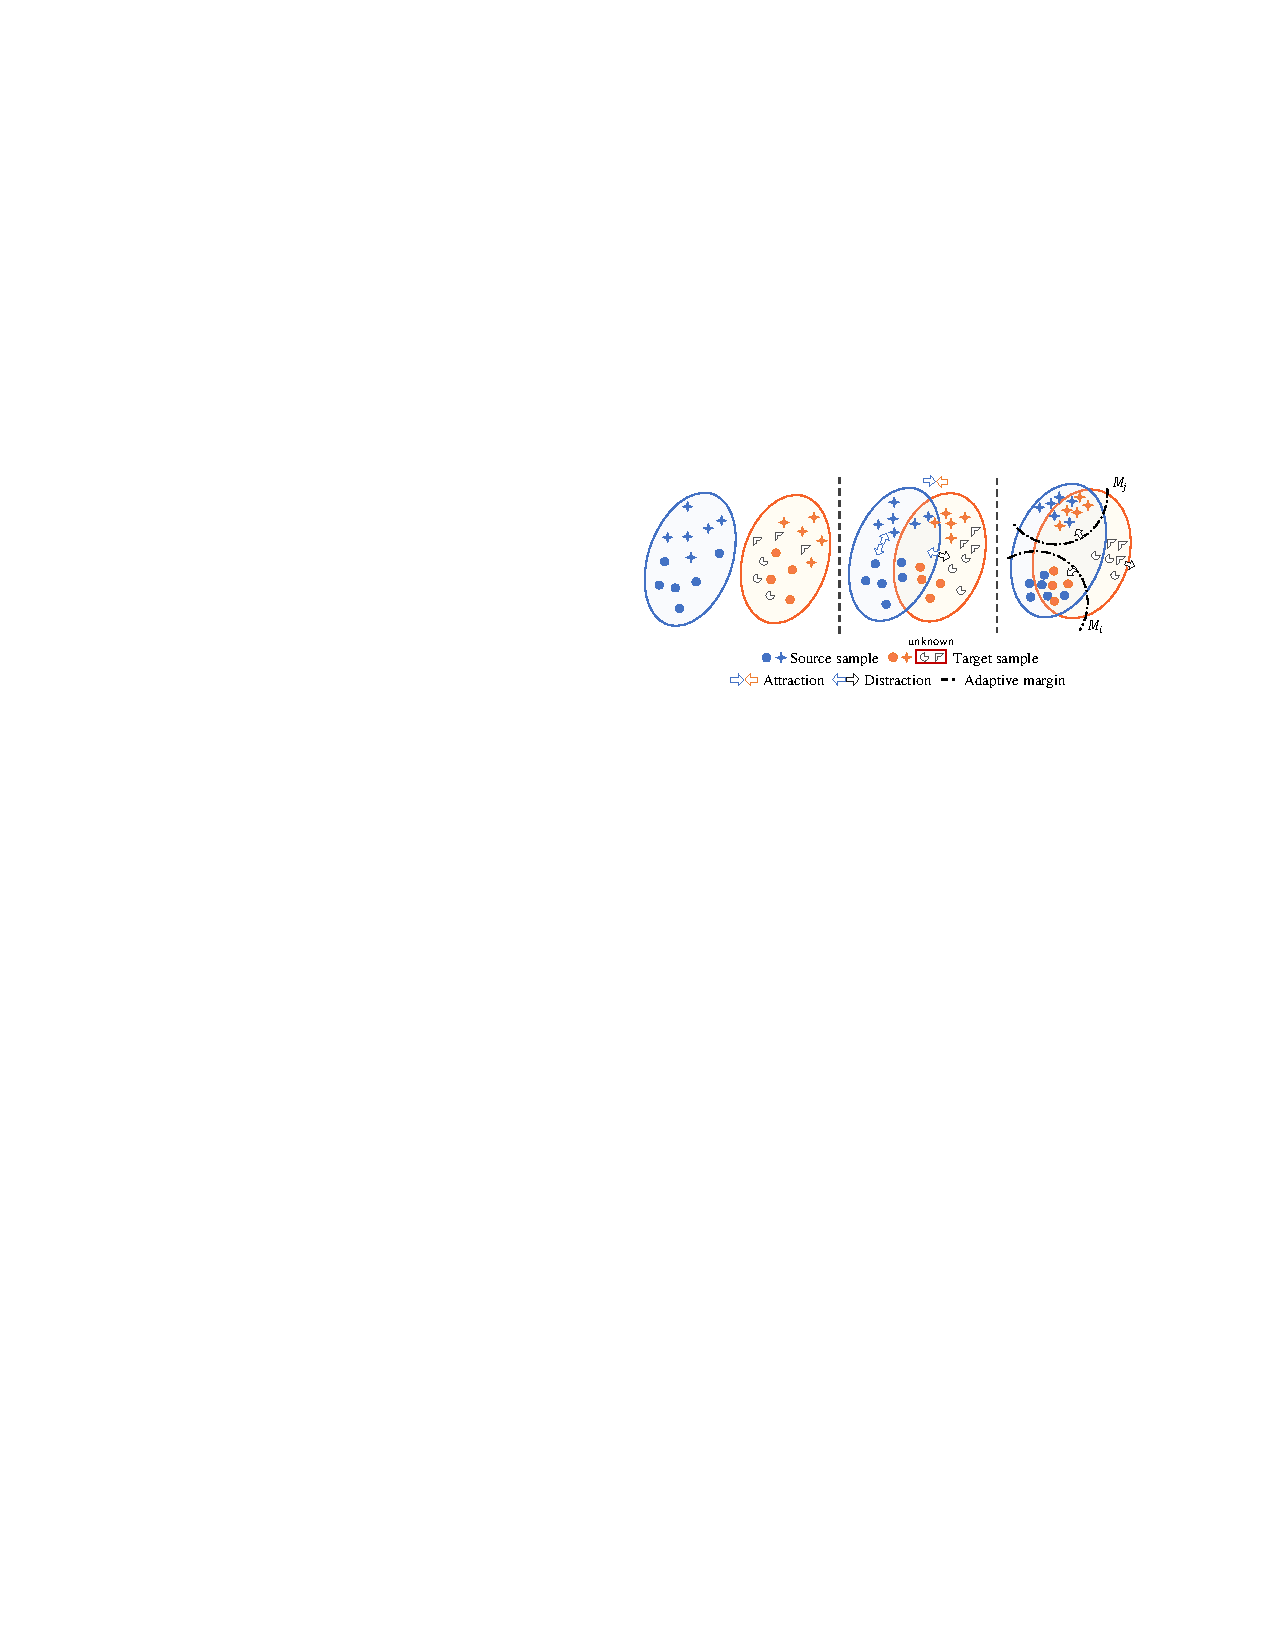
\includegraphics[width=0.52\textheight]{UDA.pdf}
	\caption{UDA算法思路\cite{1-94}}
	\label{fig1-11}
\end{figure}

考虑到基于MI范式的EEG信号存在的问题,无监督域适应算法便被应用到BCI领域中来。Chen等\cite{4-21}通过引入多注意力机制模块和域鉴别器,成功提取MI范式EEG数据的域不变特征,在三个不同公开数据集的跨时段MI辨识中取得了很好的效果。Hong等\cite{1-95}分别引入全局鉴别器和局部鉴别器对齐边缘分布,并降低条件分布差异。动态权重因子的引入使其能够有效权衡全局鉴别器和局部鉴别器的重要性,应对不同类型的数据分布。其的跨时段MI辨识分类取得了当时的最优结果。Tang等人\cite{1-96}提出了一种条件域自适应神经网络,从原始脑EEG时间序列中获取高分辨特征,其模型性能在更加严苛的跨被试MI场景下得到了验证。Zhang等人\cite{1-97}将EEG数据的协方差矩阵利用黎曼流形进行对齐,然后通过域适应算法最小化样本的联合概率分布。其在包含左手和右手两个类别的私人数据集上进行了性能验证,并击败了当时的最优算法。Zhu等人\cite{1-98}提出多源融合自适应正则化,结合加权平衡分布自适应,减少多源域间的域间差异。其挑选了公开MI数据集的左手想象和右手想象两个类别,验证了模型性能。

虽然这些方法取得了令人兴奋的结果,但是其中使用的UDA技术仍然需要改进,以应对更现实的MI应用场景。具体来说,在现实使用环境中,BCI系统常常面对同时跨被试和跨时段的应用要求,并且需要进行更多类别的分类辨识任务,这对BCI系统中的EEG解码算法提出了严峻挑战。



\section{本文的主要工作和创新点}
伴随着对大脑生理机制研究的不断深入,BCI系统的落地应用成为了可能。但是,现有基于EEG的BCI系统仍然在硬件和软件上存在着一定的不足,这制约了BCI系统在现实环境中的发展与推广。在硬件方面,当前市面上的高性能EEG采集设备存在着体积庞大,操作步骤复杂,价格昂贵的缺点,使其难以真正走入日常生活;消费级EEG采集设备又因为EEG通道数量较少,信号质量较差而限制了BCI的最终性能。因此,设计一款价格低廉,使用便捷,性能可靠,并且通道数量充足的EEG采集设备对BCI系统的发展具有重要的意义。同时,在软件方面,当前的EEG解码算法存在着结构设计困难,调参耗时以及泛化能力较差的问题。因此,本文配合采集设备,针对当前不同范式EEG信号的自身特点,对无需外部刺激诱发的被动范式和MI范式设计相应的EEG解码算法,有效推动BCI系统在情感分析、疲劳预警以及运动机能康复领域的应用。

针对当前BCI系统的不足,本课题分别从硬件和软件方面着手,设计并搭建了一套完整的BCI系统。其主要创新点如下:

(1) 本课题设计了一套基于EEG的BCI系统,命名为——JS-AINS-40。该系统的采集模块基于ARM微处理器和EEG集成前端芯片进行设计,能够以250 Hz-1000 Hz的采样率,同时采集40通道的EEG信号。为了尽可能降低采集系统中的噪声干扰,JS-AINS-40选型低噪声,高电源抑制比(Power Supply Rejection Ratio,PSRR)的供电芯片组成电源模块。同时,为了防止数字模块对模拟模块可能造成的干扰,在数字模块和模拟模块之间设计隔离模块。最后,为了提升设备在实际使用环境中的可靠性,在采集前端增加了低通滤波电路以消除EEG信号中的高频干扰,并在采集设备外露金属部分设计静电保护电路。在采集模块的硬件基础上,设计配套的下位机软件,并配合设计完成具有实时波形显示和数据保存功能的上位机软件。EEG采集硬件与下位机软件,上位机软件一同组成JS-AINS-40 BCI系统。设计完成后,本课题根据国标要求对JS-AINS-40系统进行了包括电压测量、共模抑制比测试、噪声电平测试以及电磁兼容性测试在内的性能检验,其结果符合国家标准。

(2) BCI系统的上位机不仅负责控制采集设备,接收EEG数据以及进行数据可视化,其还应具备EEG解码功能。本课题针对现有基于深度学习的EEG解码算法所存在的模型设计困难,参数调整耗时以及泛化能力不足问题,利用被动范式EEG数据量充足的优势,引入结合自适应机制和早停机制的神经结构搜索算法,成功实现了针对人脑情绪状态和疲劳状态的分类辨识。这是基于梯度的神经结构搜索技术在EEG领域的创新应用。为了验证模型的具体性能,本课题首先引入了基于情绪和疲劳的EEG公开数据集,并在其上取得了极具竞争力的分类结果。同时,为了进一步验证JS-AINS-40系统采集模块的性能,设计EEG情绪实验,并通过JS-AINS-40系统进行数据采集。最终的辨识结果验证了JS-AINS-40系统的可靠性。在两种不同类型被动范式EEG数据上的实验结果证明,所设计模型可以根据不同的数据集构建有针对性的网络架构,并具有针对基于EEG的心理生理状态识别任务的有效性和通用性。

(3) 本课题针对MI范式的EEG数据所具有的样本数量少,特征差异大问题,综合考虑MI-BCI系统所面临的使用情景,基于无监督域适应算法设计人脑运动意图辨识框架。这一框架融合动态迁移,伪标签自训练和迭代训练算法,成功实现了在MI数据上的跨被试同时跨时段分类。在三个公开MI数据集上的实验结果表明该框架具备优异的分类辨识性能。同时,配合JS-AINS-40系统,设计并进行MI实验。在JS-AINS-40所采集的数据集上的成功不仅进一步证明了所提出辨识框架的有效性,也证明了JS-AINS-40系统的可靠性。在四个MI数据集上,本课题验证了所提出框架的设计合理性,并对各模块的超参数选取进行了详细分析。

\section{本文工作的结构安排}

第一章~绪论

本章主要介绍了本课题的研究背景及意义,并从基于EEG的BCI系统基本结构和应用领域、EEG信号的基本特征,基于EEG的BCI系统典型范式以及国内外EEG采集设备的发展情况综合介绍基于EEG的BCI系统的研究现状。同时,本章还介绍了基于深度学习技术的EEG信号分析,以及深度学习的两个分支——神经架构搜索技术和无监督域适应算法的发展现状及其在EEG领域上的应用。最后,总结了本文的主要工作和创新点。

第二章~脑电信号采集系统设计

本章引入并介绍了JS-AINS-40系统。本章首先介绍了BCI系统应当具备的设计指标,并说明了JS-AINS-40系统的整体框架。其次,分别从硬件和软件两个方面展开介绍。硬件部分,本章首先介绍了JS-AINS-40系统的外观结构,并说明了其中两个组成部分——EEG采集盒和脑电极帽的外形参数。接下来,依次介绍了EEG采集盒中采集模块电路的各子模块器件选型以及电路设计。软件部分,本章分别介绍了JS-AINS-40系统的下位机软件设计流程以及上位机软件具体功能。最后,本章说明了对JS-AINS-40系统进行的性能测试,并展示了测试结果。

第三章~基于梯度自动优化的脑电辨识模型

本章介绍了JS-AINS-40系统配套的,针对被动范式中情绪和疲劳EEG的解码算法。首先,本章说明了根据EEG类型所引入的特征提取方法,介绍了所设计模型的基础架构,并在此基础上,详细说明了为了将基于图像的神经架构搜索技术迁移至EEG数据,所进行的针对性改进。其次,本章介绍了用来验证模型性能的情绪和疲劳两款公开数据集,以及用来验证JS-AINS-40可靠性的情绪数据集的具体采集流程。最后,本章分别介绍了所提出算法在三个数据集上搜索得到的最终模型架构,以及其分类辨识性能。通过与其他EEG辨识算法和神经架构搜索算法进行比较,验证了所提出模型的优异性。

第四章~基于多被试动态迁移与迭代自训练的脑电辨识算法

本章介绍了JS-AINS-40系统配套的,针对主动范式中MI类型EEG的解码算法。本章首先说明了常规算法在MI数据上存在的问题,申明了本章所提出框架的必要性。其次,定义了所提出框架应用的具体情景,并在此基础上详细介绍了框架的内部构成。接下来,本章说明了用来评估模型性能所使用的数据集,以及利用JS-AINS-40采集MI数据集的具体实验流程。除了数据集外,还介绍了所设计的对比算法,以及本章进行性能验证时的具体实验设定。紧接着,本章给出了所提出框架以及所有对比算法在四个MI数据集上的辨识结果,并对比了所有方法的复杂度。最后,通过大量的消融实验,本章证明了所提出框架设计的合理性,并对超参数选取进行了解释。

第五章~总结与展望

本章总结了全文的主要工作内容,并对未来该工作可能的研究方向进行展望。
